% ================================================================
% CHAPTER 4: Lösung
% ================================================================

	
\chapter{Lösung}

\section{Codierung von Domänenwissen}

Tabelle xx (<<VERWEIS AUF TABELLE EINFÜGEN>>) codiert Domänenwissen von Tierärzten, welches für die Geburtsprognose von Bedeutung ist. Expertenwissen ist so codiert, dass jedes Geburtsmerkmal mit einer Gewichtung versehen ist. Somit hat das Merkmal an Stelle $i$ die Gewichtung $\lambda_{i}$.



Wie in Formel \ref{Linerarkombination zur Geburtsprognose} formalisiert, werden bei Erkennung eines oder mehrerer Merkmale in einem Bild, die Gewichtungen dieser Merkmale addiert. Merkmale, welche als Geburtsanzeichen dienen, haben eine positive Gewichtung und erhöhen dadurch das Endergebnis. Merkmale, welche darauf hinweisen, dass zurzeit keine Entbindung stattfindet, haben eine negative Gewichtung und senken das Endergebnis.


Das Resultat dieser Berechnung bezeichnet der Autor als \flqq qualitative Situationsbewertung\frqq. Diese wird mit einem Schwellwert verglichen, um zu entscheiden, ob eine Benachrichtigung verschickt wird.

Dabei kann die qualitative Situationsbewertung anhand der folgenden Linearkombination ermittelt werden: 



\begin{equation}\label{Linerarkombination zur Geburtsprognose}
v = h(x) = \sum_{i=1}^n \lambda_{i}*x_{i}
\end{equation}

 
Wobei $\lambda_{i}$ sich aus der fachlichen Gewichtung $\kappa_{i}$ und der technischen Qualitätsbeurteilung $\beta_{i}$ zusammensetzt. Die Skala zur Bewertung reicht von -10 bis 10, daher ergibt sich $ \lambda = \kappa = \beta = \{ \:  m \: | \:  m \:  \varepsilon \:  \mathbb{Z}, -10 \:  \leq \: m \: \leq \:  10\} $.

Die fachliche Gewichtung eines Merkmals entspricht der Bewertung  der Stärke des Hinweises in Bezug auf eine bevorstehende Geburt. Dementsprechend codiert $\kappa$ Domänenwissen von Tierärzten zur merkmalsbezogene Einschätzung und Prognose des Geburtsverlaufs.

Die technische Qualitätsbeurteilung basiert auf der Güte der technischen Mittel zwecks Analyse der An- oder Abwesenheit eines Merkmals in einem Bild. Dementsprechend wird $\beta$ benötigt, weil nicht sämtliche Merkmale mit derselben Qualität auf deren An- oder Abwesenheit überprüft werden können.

Zwischen den beiden Gewichtungen $\kappa$ und $\beta$ existiert eine schwache Beziehung. Dies wird dadurch begründet, dass technische Zuverlässigkeit die Anwesenheit eines Merkmals nicht überbewerten soll. Beispielsweise soll eine besonders hohe technische Qualitätsbeurteilung und eine tiefe fachliche Gewichtung nicht in einer hohen Gewichtung resultieren. Um diese zwei Gewichtungen schwach miteinander in Beziehung zu setzen, werden diese addiert und nicht multipliziert. Es gilt also: $\lambda_{i} = \kappa_{i} + \beta_{i}$

Zudem codiert $x_{i}$ die Anwesenheit ($x_{i}=1$) oder die Abwesenheit ($x_{i}=0$) eines spezifischen Merkmals auf einem Bild. Es gilt dementsprechend  $ x_{i} \:  \varepsilon \: \{0,1\}. $ 


Setzen wir diese Erkenntnisse zusammen, so ergibt sich

\begin{equation}\label{Vollständige Linerarkombination zur Geburtsprognose}
v = h(x) = \sum_{i=1}^n (\kappa_{i}+\beta_{i}) *x_{i}
\end{equation}

wobei:  $ x \:  \varepsilon \: \{0,1\} $ und $\kappa = \beta = \{ \:  m \: | \:  m \:  \varepsilon \:  \mathbb{Z}, -10 \:  \leq \: m \: \leq \:  10\} $.

Das Ergebnis dieser Rechenoperation ergibt wie bereits erwähnt die qualitative Situationsbewertung $v$, welche mit einem Schwellwert verglichen wird. Dies wird formal wie folgt ausgedrückt:

\begin{equation}\label{Vollständige Linerarkombination zur Geburtsprognose: Schwellwertanalyse}
y = g(v) =\begin{cases}
			1,\: wenn \: v > q\\
			0,\: wenn \: v \leq q
\end{cases}
\end{equation}

Dabei steht $q$ für den Schwellwert, welcher in der Domänenanalyse ermittelt wird. Das Ergebnis $y=1$ bedeutet, dass eine Benachrichtigung ausgelöst wird, während bei $y=0$ keine Benachrichtigung ausgelöst wird.

 






\newgeometry{margin=2.5cm} % Ränder kleiner	
\begin{landscape}

\section{Modellierung der Lösung}
Für die Dokumentation der Lösung verwendet der Autor die UML-Notation. Zwei Kassendiagramme beschreiben das System aus jeweils unterschiedlichen Perspektiven \cite{Uml-modellierung2012}. 

\subsection{Klassendiagramm des Pakets Image-Analysis }
\begin{figure}[H]
	\center
	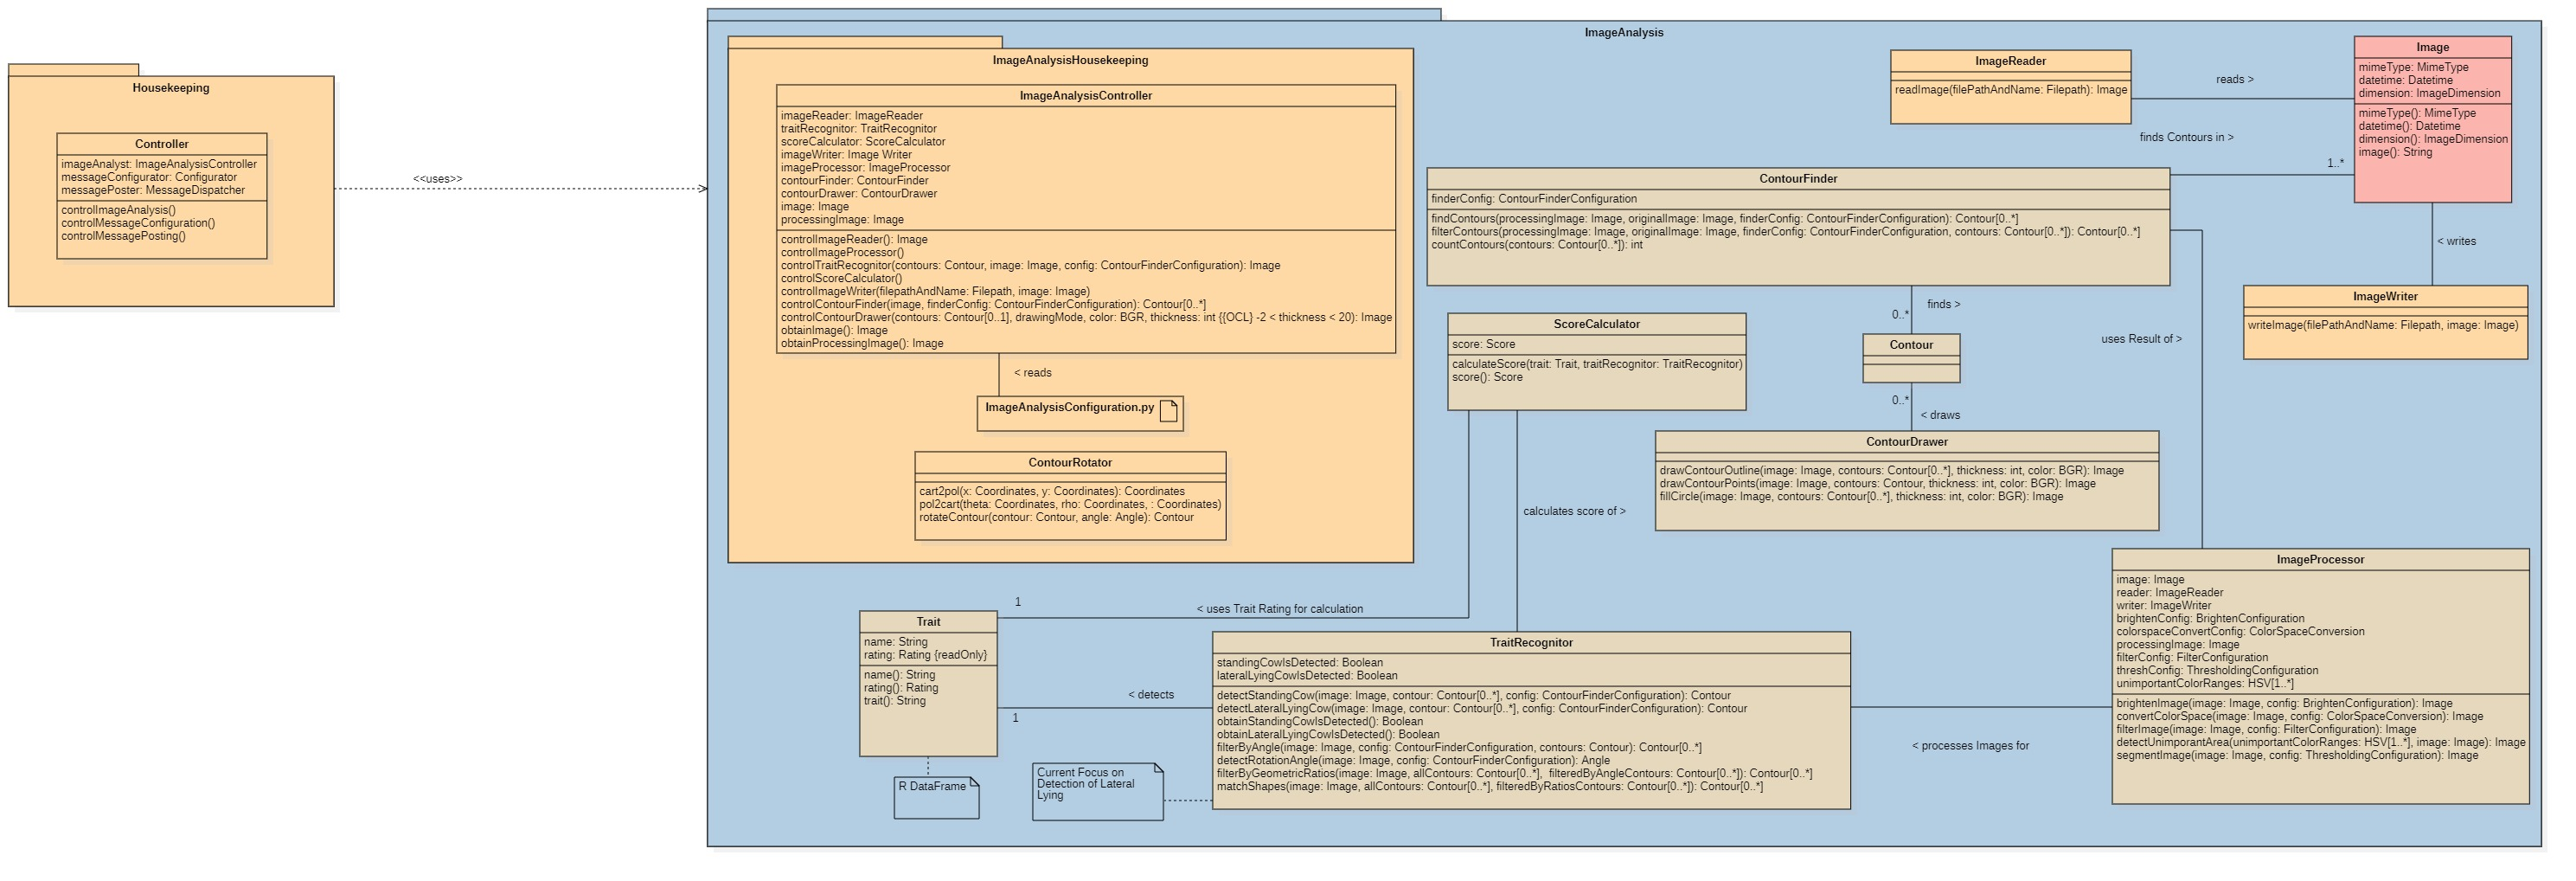
\includegraphics[scale=0.45]{Grafiken/modelle/solution-imageanalysis.jpg}
	\caption{Lösungsdokumentation des Pakets Image-Analysis zur Geburtsprognose und Geburtserkennung.} 
	\label{fig: Lösungsdokumentation des Pakets Image-Analysis zur Geburtsprognose und Geburtserkennung.}
\end{figure}

\subsection{Klassendiagramm der Pakete Message-Configuration und Message-Posting}
\begin{figure}[H]
	\center
	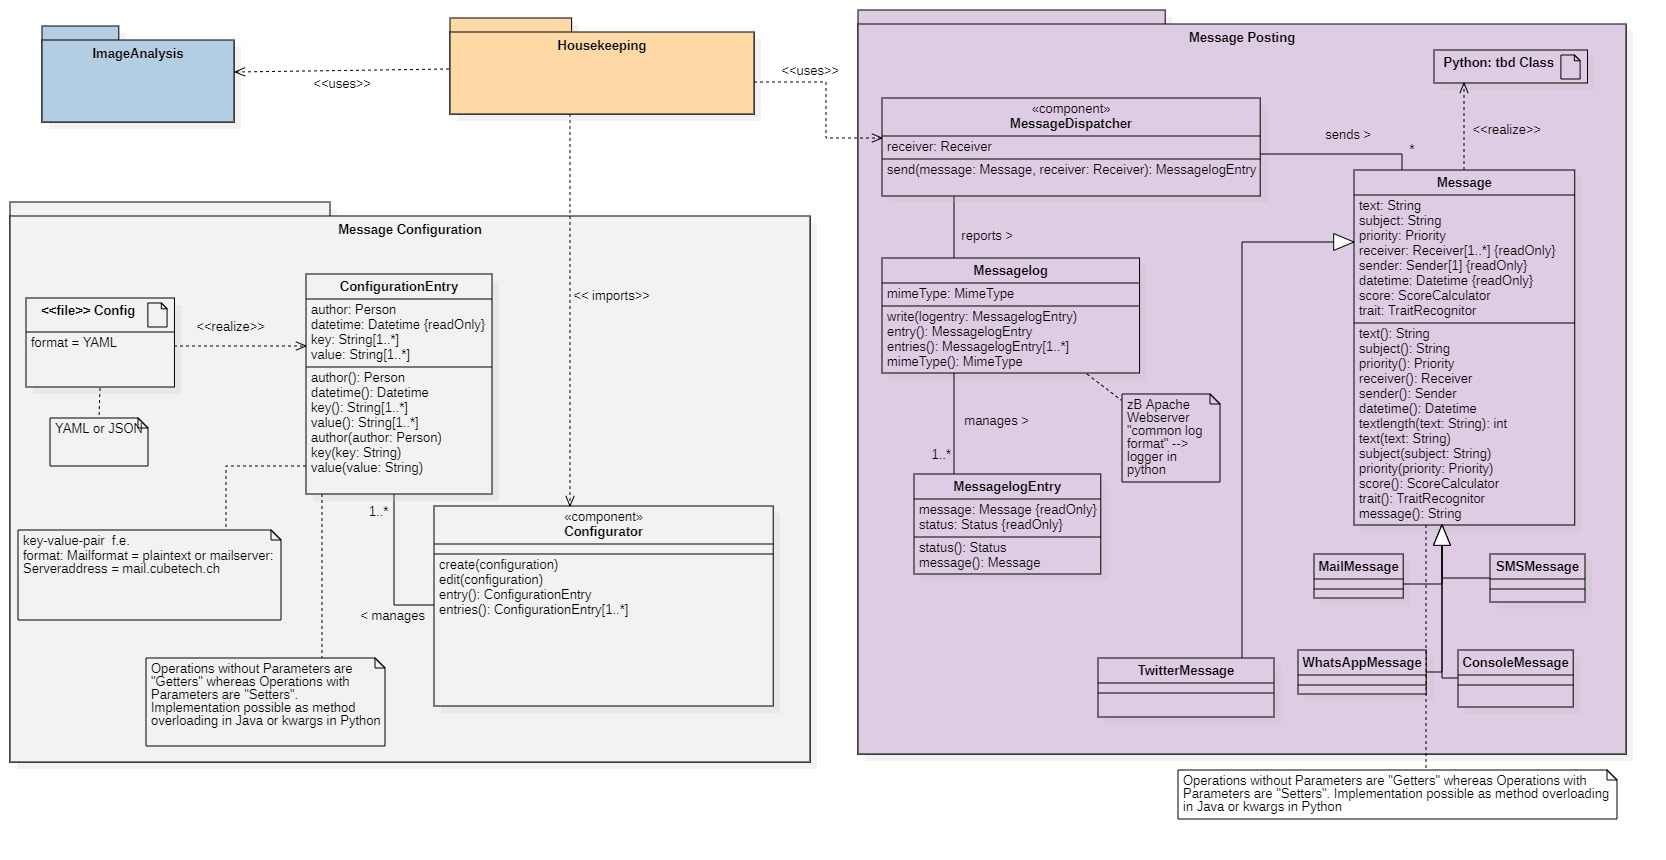
\includegraphics[scale=0.43]{Grafiken/modelle/solution-messaging.jpg}
	\caption{Lösungsdokumentation der Pakete Message-Configuration zur Konfiguration und Message Posting zum Versand von Benachrichtigungen.} 
	\label{fig: Lösungsdokumentation der Pakete Message-Configuration zur Konfiguration und Message Posting zum Versand von Benachrichtigungen.}
\end{figure}

\subsection{Value-Object-Bibliothek}
Die Bibliothek an Value Objects wird gemäss Kapitel 3 Domänenanalyse eingesetzt.

Zusammenfassend ist erwähnenswert,... 

\end{landscape}
\restoregeometry % Wieder die alten Ränder

\section{Überlegungen für den Betrieb}

Um einen stabilen Betrieb von elektronischen Geräten und dem Netzwerk auf einem Bauernhof sicherzustellen, müssen folgende Überlegungen gemacht werden:


\newpage


\section{Umsetzung in Entwicklung}
Für Bildanalysen sind grundsätzlich Methoden des Machine Learning geeignet. Da für die vorliegende Arbeit jedoch nicht auf eine grosse Menge von klassifizierten Bildern zugegriffen werden kann, wird die Bildanalyse auf Basis von geometrischen Eigenschaften durchgeführt.
Um die schrittweise Entwicklung und entsprechende Teilergebnisse der Bildbearbeitung zu veranschaulichen, dient Abbildung \ref{fig: Ausgangslage für die Bildanalyse} als Ausgangsbild. Dieses Bild wurde vom System erstellt, welches im Rahmen der erwähnten Case-Arbeit entwickelt wurde. Anschliessend wurde das Bild mit der Funktion \texttt{add()} heller gemacht und unter Anwendung von \texttt{createCLAHE()} und \texttt{clahe.apply()} wurde das Histogramm des Bildes geglättet. 

\begin{figure}[H]
	\center
	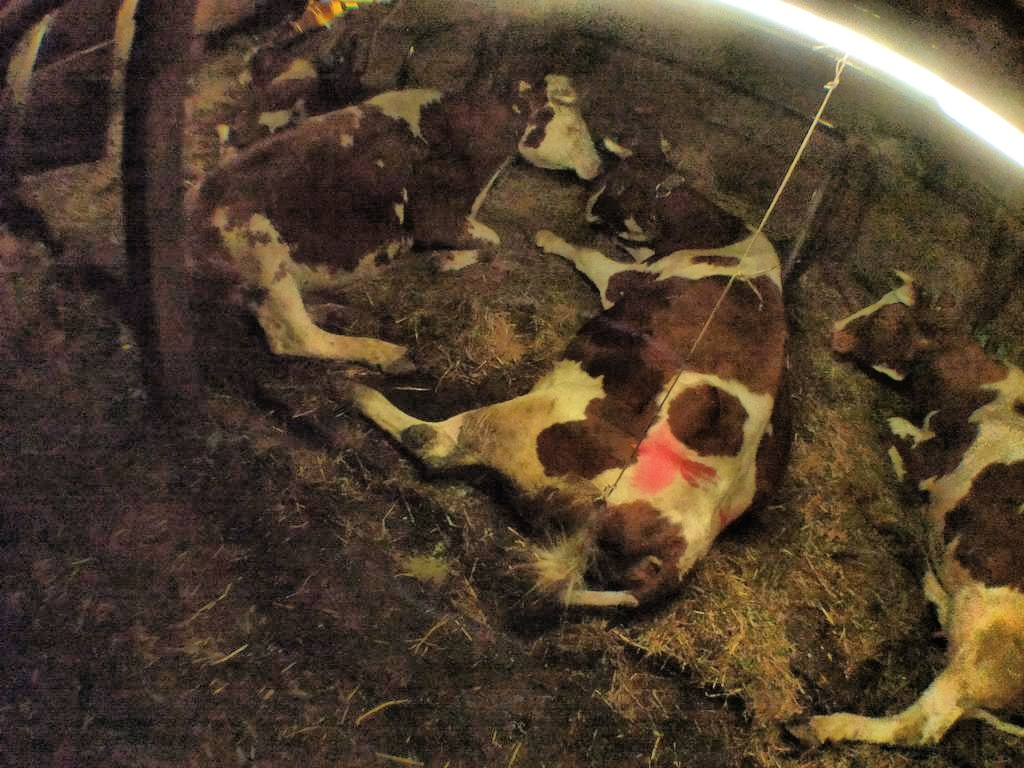
\includegraphics[scale=0.43]{Grafiken/entwicklung/1ausgangsbildBericht.jpg}
	\caption{Beispielbild als Ausgangslage zur Veranschaulichung des Vorgehens} 
	\label{fig: Ausgangslage für die Bildanalyse}
\end{figure}

Abbildung \ref{fig: Vergleich der Histogramme vor und nach Bildbearbeitung} zeigt auf der linken Seite das Histogramm des Originalbilds und auf der rechten Seite das Histrogramm des aufgehellten und geglätteten Bilds. Dabei fällt auf, dass aufgrund der Aufhellung des gesamten Bildes im Histogramm der Wertebereich nach rechts verschoben wird. Zudem sind als Folge der Glättung des Histogramms mittels CLAHE\footnote{Contrast Limited Adaptive Histogram Equalization} die Anzahl Pixel weniger stark auf einen Bereich konzentriert. CLAHE ist ein Verfahren, dass für die Glättung von Bildern und Verbesserung des Kontrasts eingesetzt wird. Ein Vorteil der Methode ist, dass aufgrund einer parametrisierbaren Begrenzung der Kontrastverstärkung die Überbetonung von Rausch in relativ homogenen Regionen des Bilds verhindert wird \citep[S. 313]{FernandezVillan2019}.

Das Bild \ref{fig: Ausgangslage für die Bildanalyse} wird nun unter Anwendung von diversen Methoden aus der Bildanalyse und der Software-Bibliothek OpenCV bearbeitet und analysiert, um daraus Information zum Geburtsverlauf eines Kalbes zu gewinnen. In der vorliegenden Arbeit liegt der Fokus in der Detektierung von seitlichem Liegen, da die Erkennung dieses Geburtsmerkmals einen hohen Mehrwert bringt. 

\begin{figure}[H]
	\center
	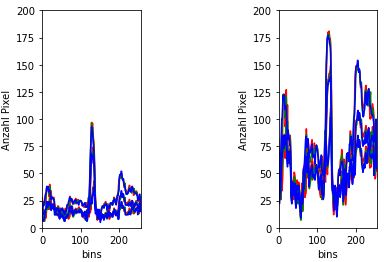
\includegraphics[scale=0.9]{Grafiken/entwicklung/2HistrogrammVergleich.jpg}
	\caption{Vergleich der Histogramme vor und nach Bildbearbeitung} 
	\label{fig: Vergleich der Histogramme vor und nach Bildbearbeitung}
\end{figure}

\subsection{Detektierung von unwichtigen Bereichen im Bild}
Um das Potential aus der Detektierung von unwichtigen Bereichen zu veranschaulichen, wird in einem ersten Schritt ein Binärbild des Originalbilds erstellt. Dazu wird die Funktion \texttt{threshold()} mit dem Verfahrentyp \texttt{THRESH_BINARY} und dem Wert \texttt{90} als Schwellwert eingesetzt. OpenCV ermöglicht mit der Funktion \texttt{threshold()}, die Segmentierung des Bilds. Dabei wird dieses in eine Repräsentation umgewandelt, welche sich für die Weiterverarbeitung besser eignet als die ursprüngliche. \cite[S.328-335]{FernandezVillan2019} In der vorliegenden Arbeit basiert die Extraktion von Objekten darauf, dass durch Schwellwertverfahren bestimmte Eigenschaften wie Farben und Ecken erkannt werden können und dadurch mittels Parition des Bildes zwischen Vorder- und Hintergrund unterschieden werden kann. Die Auswahl vom Wert \texttt{90} als Schwellwert hat zur Folge, dass Pixel mit einer Intensität kleiner gleich \texttt{90} im resultierenden Bild schwarz dargestellt werden und alle anderen Pixel weiss. Gleichung \ref{Schwellwertanalyse} verdeutlicht die Folge der Parametrisierung von \texttt{threshold()} in der vorliegenden Arbeit. 

\begin{equation}\label{Schwellwertanalyse}
dst(x,y) =\begin{cases}
255,\: if \: src(x,y) > 90\\
0\: otherwise
\end{cases}
\end{equation}

Als Bild zur Eingabe dient ein Graustufenbild. Grundsätzlich können mithilfe des Parameters \texttt{maxval} bei Erreichung des Schwellwerts auch Graustufen als Zielwert für Pixel zugewiesen werden. Da in der vorliegenden Arbeit das Schwellwertverfahren aber in erster Linie zur Vorbereitung für \texttt{findContours()} gemacht wird, bringt ein Bild in Graustufen keinen Mehrwert. Die Funktion \texttt{findContours()} weist sämtlichen Pixeln, die nicht den Wert \texttt{0} haben, den Wert \texttt{1} zu. Dementsprechend wird auch ein Bild mit Graustufen als Binärbild behandelt \cite[S. 366]{FernandezVillan2019}. 



Nebst der Funktion \texttt{threshold()} und dem Typ \texttt{THRESH_BINARY} bietet OpenCV weiteren Typen wie \texttt{THRESH_BINARY_INV} oder \texttt{THRESH_TRUNC} und das adaptive Schwellwertverfahren \texttt{adaptiveThreshold()} an. Adaptive Schwellwertverfahren ermöglichen den Einsatz von spezifischen Schwellwerten für einen Pixel im Zielbild. Dieser spezifische Schwellwert wird auf Basis einer Gruppe von benachbarten Pixeln  ermittelt \cite[S.342 f]{FernandezVillan2019}. Die im Rahmen der Bachlor-Arbeit entwickelte Lösung unterstützt die Parametrisierung dieser Funktionen mittels Enumerations. Diese haben für die vorliegende Bildanalyse jedoch keine zentrale Bedeutung und werden deshalb nicht weiter erläutert.

\begin{figure}[H]
	\center
	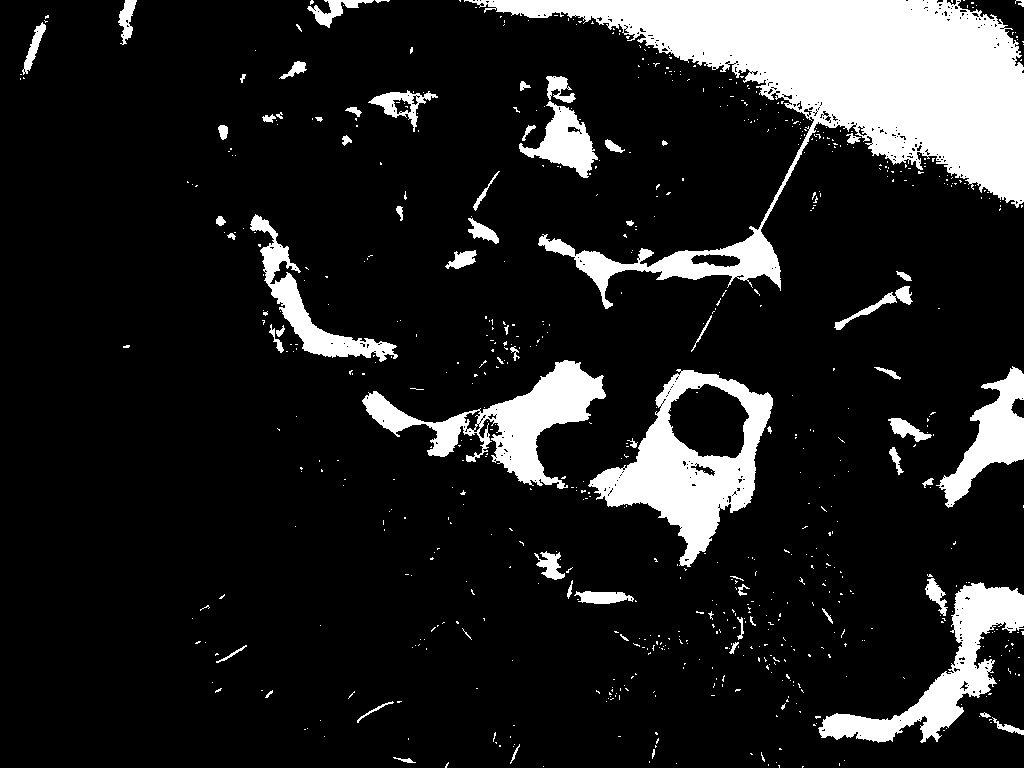
\includegraphics[scale=0.43]{Grafiken/entwicklung/8thresholdedMask.jpg}
	\caption{Binärbild als Resultat vom Schwellwertverfahren} 
		\label{fig: Binärbild als Resultat vom Schwellwertverfahren}
\end{figure}
		
Im Binärbild aus Abbildung \ref{fig: Binärbild als Resultat vom Schwellwertverfahren} werden anschliessend mit den Funktionen \texttt{findContours()} und \texttt{drawContours()} Konturen gesucht und im Originalbild eingezeichnet. Die Funktion \texttt{findContours()} wird verwendet, um Konturen in einem Binärbild zu erkennen. Der Algorithmus unterstützt unterschiedliche Modi wie \texttt{RETR_EXTERNAL} für die Beschränkung auf äussere Konturen, \texttt{RETR_LIST} für die Ausgabe sämtlicher Konturen ohne Hierarchie oder \texttt{RETR_TREE} für die zusätzliche Ausgabe von Informationen zur Hierarchie der Konturen \cite[S.366]{FernandezVillan2019}. In der vorliegenden Arbeit wurde in erster Linie der Verfahrenstyp \texttt{RETR_EXTERNAL} verwendet. Abweichungen werden entsprechend erwähnt.

\begin{figure}[H]
	\center
	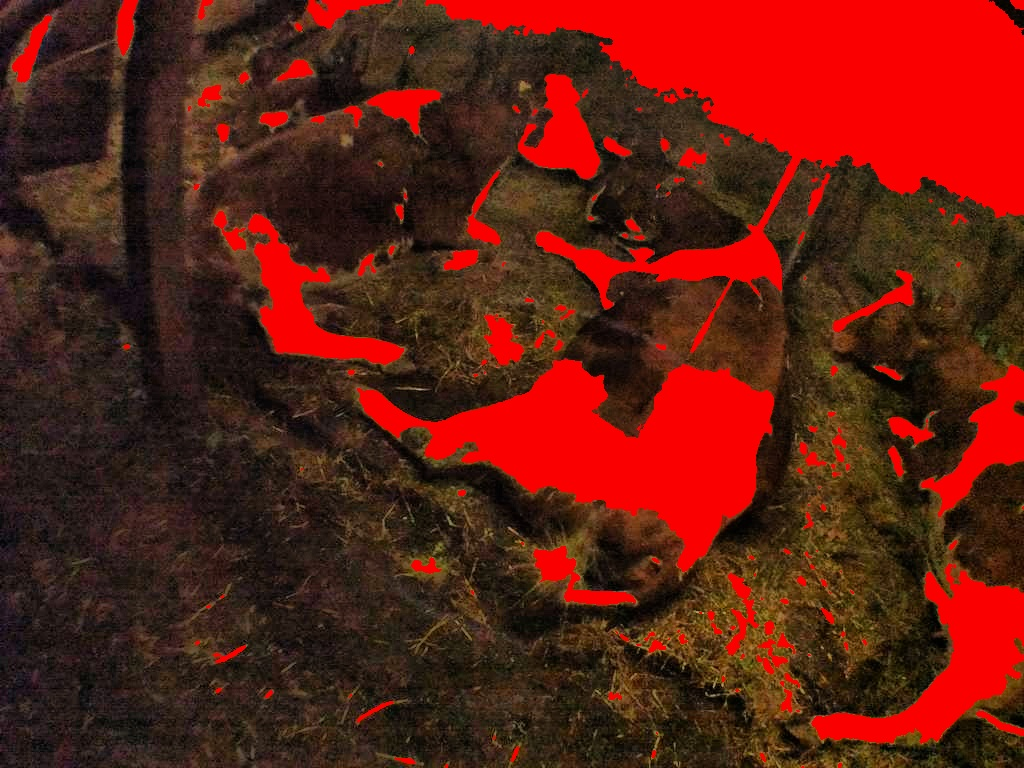
\includegraphics[scale=0.43]{Grafiken/entwicklung/8thresholdedImageAllContours.jpg}
	\caption{Originalbild mit sämtlichen Konturen rot eingefärbt} 
	\label{fig:Originalbild mit sämtlichen Konturen rot eingefärbt } 
\end{figure}

Die Anwendung der Funktion \texttt{findContours()} ohne Einschränkung der zu analysierenden Bereiche in Abbildung \ref{fig:Originalbild mit sämtlichen Konturen rot eingefärbt} verdeutlicht, dass viele Konturen eingezeichnet werden, die sich von den Konturen der Kuh stark unterscheiden. Im vorliegenden Bild betrifft dies in erster Linie die Lampe und Strohhaufen. Der Autor setzt sich daher zum Ziel, unwichtige Bereiche im Bild zu identifizieren. Dies umfasst Bereiche, welche mit hoher Wahrscheinlichkeit nicht Teile einer Kuh oder eines Kalbs zeigen. Die Farbwerte dieser Teile im Bild
unterscheiden sich stark von den meisten Farben im Kuhfell. 

Die Strohhaufen und Schatten unterhalb des Schwanzes oder unterhalb der Beine der Kuh werden ganz einfach gefiltert, indem nur Konturen mit einer Fläche von mehr als 1250 Pixel berücksichtigt werden. Daraus entsteht Abbildung \ref{fig:Originalbild mit rot eingefärbten Konturen, falls Fläche über 1250 Pixel}.

\begin{figure}[H]
	\center
	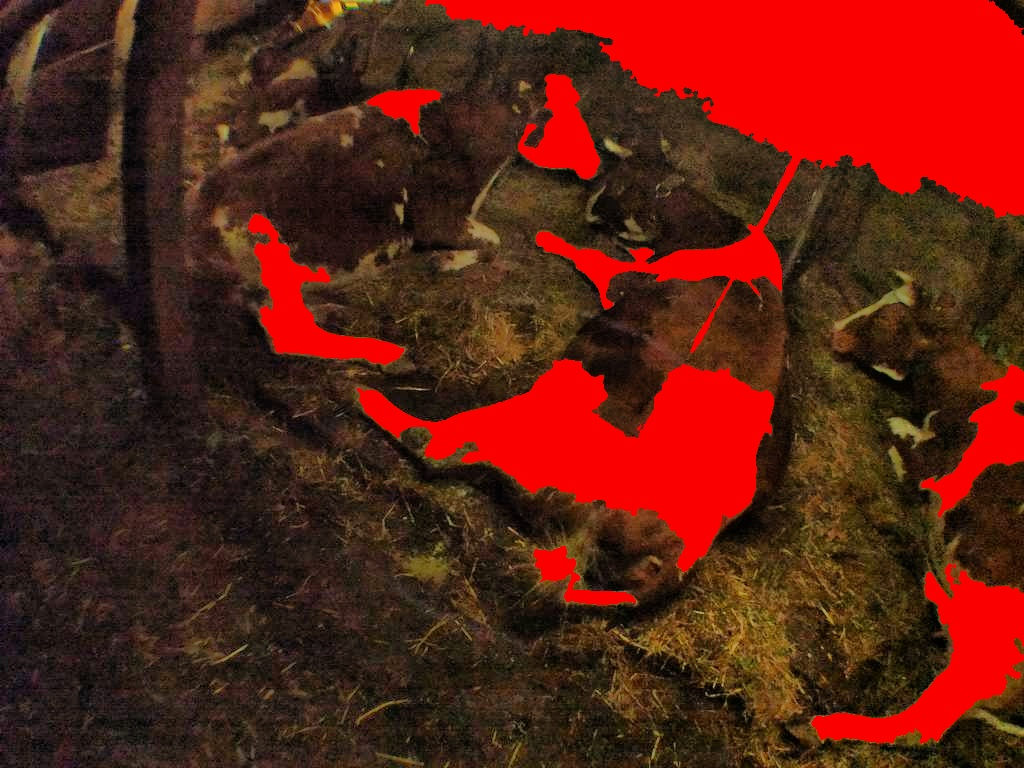
\includegraphics[scale=0.43]{Grafiken/entwicklung/9thresholdedImage.jpg}
	\caption{Originalbild mit rot eingefärbten Konturen mit Fläche über 1250 Pixel} 
	\label{fig:Originalbild mit rot eingefärbten Konturen, falls Fläche über 1250 Pixel} 
\end{figure}

Um weitere, unwichtige Konturen wie die Lampe zu erkennen, wird ein Verfahren zur Analyse von Farbwerten durchgeführt.
Dabei wird in einem ersten Schritt ein Farbbereich für die Lampe definiert. Um einen Richtwert für diesen Farbwert zu erhalten, wird mithilfe des Grafikprogramms GIMP (Version 2.10, \url{www.gimp.org}) ein Farbwert im Bereich der Lampe ausgelesen. Auf Basis dieses Richtwerts wird anschliessend ein Wertebereich für die Farbwerte der zu identifizierenden Lampe festgelegt. Diese Schwellwerte werden der Funktion \texttt{inRange()} von OpenCV zwecks Erstellung eines Binärbilds übergeben. Sämtliche Bereiche mit Farbwerten, die sich zwischen den definierten Schwellwerten befinden, werden im resultierenden Bild weiss dargestellt. Diese entsprechen unwichtigen Bereichen im Bild. Alle anderen Bereiche sind im erstellen Binärbild schwarz dargestellt. Abbildung \ref{fig: Binärbild stellt den Bereich der Lampe weiss dar} zeigt das Binärbild, welches aus diesem Verfahren entsteht. Es ist klar zu erkennen, dass die Bereiche der Lampe weiss und übrige Bereiche schwarz sind. Der Ansatz der Schnur, mit welcher der Schwanz der Kuh an der Decke befestigt wird, ist ebenfalls erkennbar. 




\begin{figure}[H]
	\center
	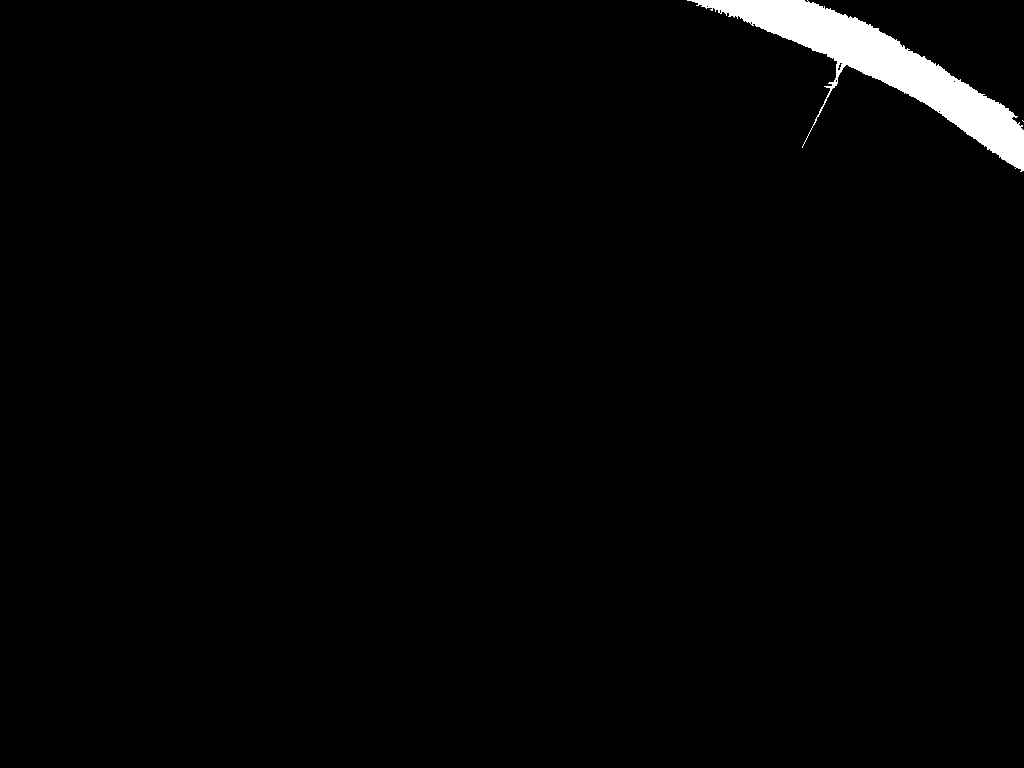
\includegraphics[scale=0.25]{Grafiken/entwicklung/3binBildLampe.jpg}
	\caption{Binärbild stellt den Bereich der Lampe weiss dar} 
	\label{fig: Binärbild stellt den Bereich der Lampe weiss dar}
\end{figure}

Dasselbe Vorgehen wird angewendet, um den Bereich des Stallbodens und Holzträgers zu identifizieren. Das erstellte Binärbild identifiziert auch einige dunkle Regionen im Deckenbereich als unwichtig. Das Ergebnis ist in Abbildung \ref{fig: Binärbild zeigt den Bereich des Stallbodens und Holzträgers} abgebildet.
\begin{figure}[H]
	\center
	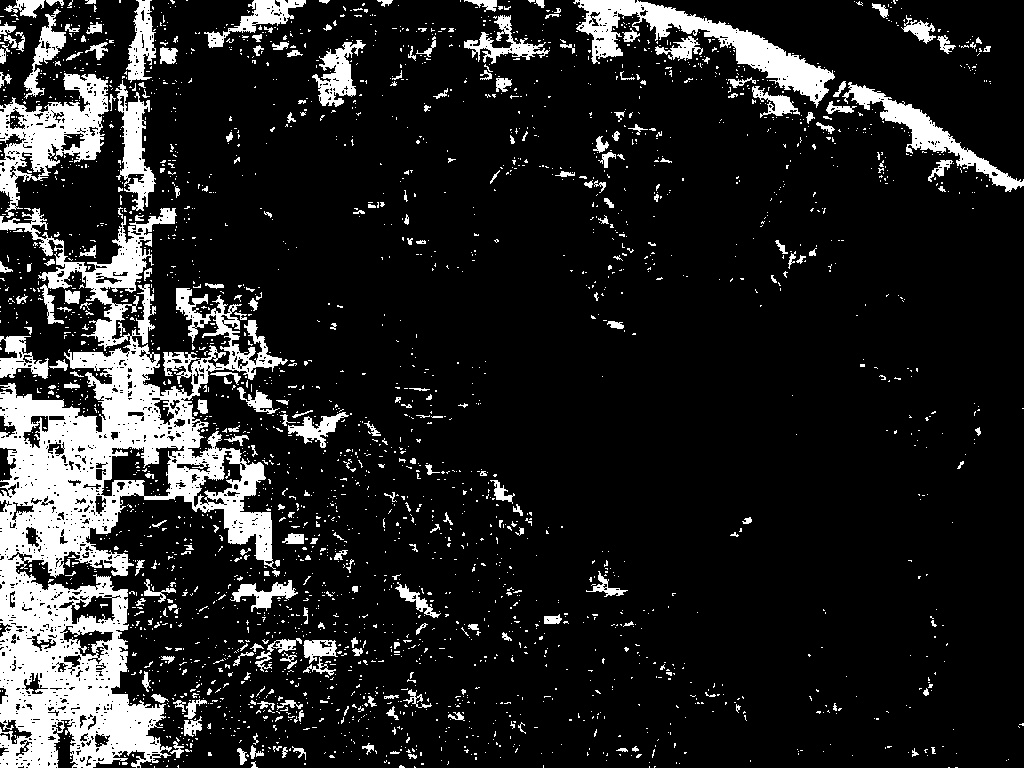
\includegraphics[scale=0.25]{Grafiken/entwicklung/4binBildHolz.jpg}
	\caption{Binärbild zeigt den Bereich des Stallbodens und Holzträgers} 
	\label{fig: Binärbild zeigt den Bereich des Stallbodens und Holzträgers}
\end{figure}

Diese zwei Binärbilder werden nun mit dem Ziel weiterverarbeitet, ein Binärbild zu erstellen, welches möglichst viele unwichtige Regionen weiss darstellt. Durch die Funktion \texttt{bitwise_or} werden die Bilder so verknüpft, dass im resultierenden Bild sämtliche Bereiche weiss sind, die in einem der beiden oder in beiden Eingangsbildern weiss sind.
\begin{figure}[H]
	\center
	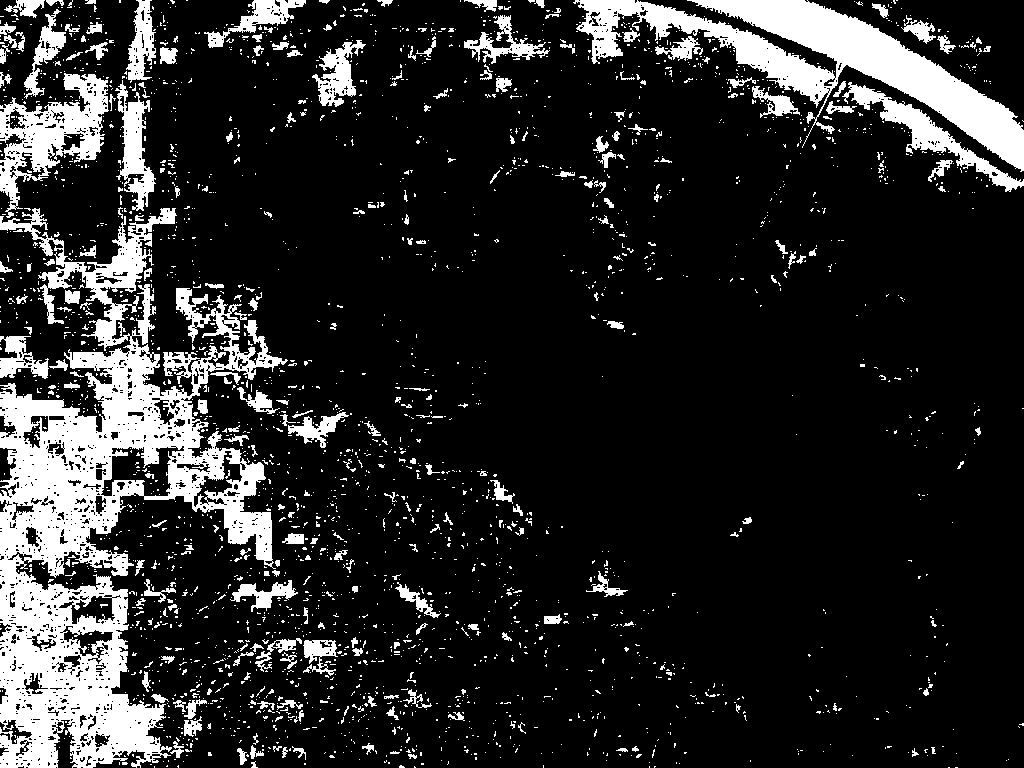
\includegraphics[scale=0.25]{Grafiken/entwicklung/5binLampeUndHolz.jpg}
	\caption{Binärbild zeigt die als unwichtig identifizierten Bereiche} 
	\label{fig: Binärbild zeigt sämtliche als unwichtig identifizierten Bereiche}
\end{figure}

Ausgehend von Abbildung \ref{fig: Binärbild zeigt sämtliche als unwichtig identifizierten Bereiche} können die als unwichtig identifizierten Bereiche als Konturen erkannt und im Originalbild eingezeichnet werden. Um dies zu erreichen, werden die Funktionen \texttt{findContours()} und \texttt{drawContours()} wie bereits erwähnt angewendet. Das Resultat ist in Abbildung \ref{fig: Unwichtige Bereiche als Konturen} veranschaulicht. 
\begin{figure}[H]
	\center
	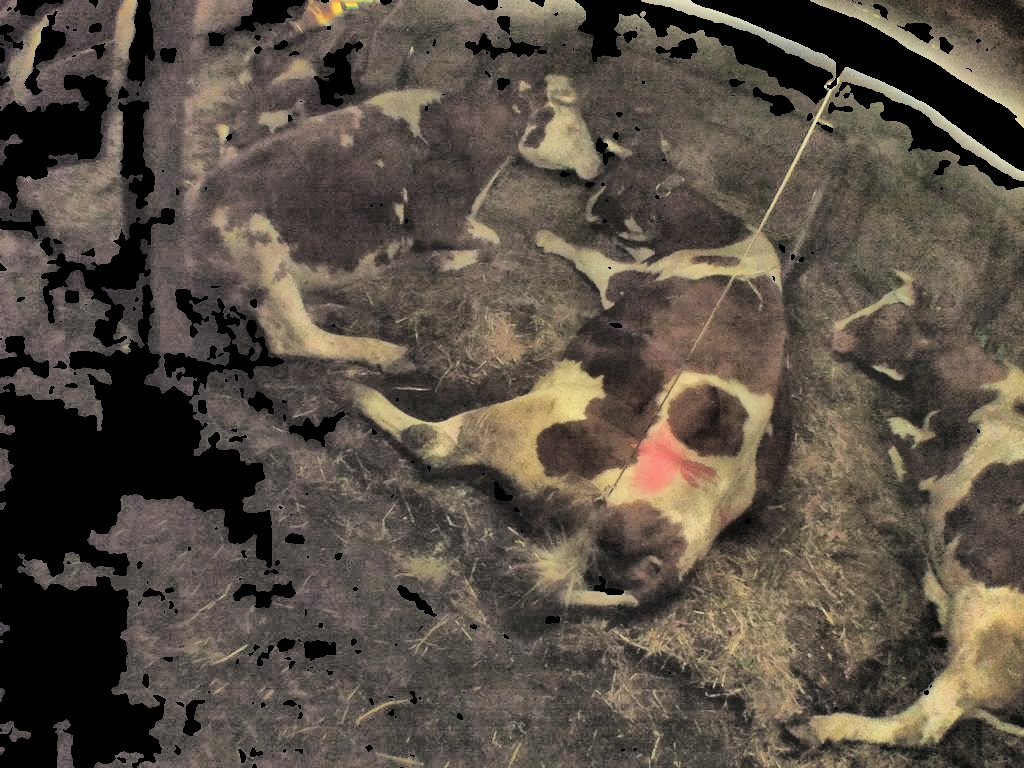
\includegraphics[scale=0.43]{Grafiken/entwicklung/6unwichtigeBereicheEingezeichnet.jpg}
	\caption{Unwichtige Bereiche  als Konturen} 
	\label{fig: Unwichtige Bereiche als Konturen}
\end{figure}

Nun gilt es, auf Basis der als unwichtig identifizierten Konturen möglichst grosse Flächen aus dem Originalbild zu entfernen, respektive möglichst grosse Flächen mit schwarzer Farbe zu füllen. Um dies zu erreichen, werden mehrere Verfahren getestet. Die Abbildungen  \ref{fig: Unwichtige Bereiche als Polygone} bis \ref{fig: Unwichtige Bereiche als Rechtecke} veranschaulichen die entsprechenden Resultate unter Verwendung von OpenCV. 

In Abbildung \ref{fig: Unwichtige Bereiche als Polygone} wurde \texttt{approxPolyDP()} verwendet, um basierend auf den Konturen ein Vieleck zu approximieren. Die Funktion arbeitet nach dem Douglas-Peucker-Algorithmus, welcher aus einer gegebenen Kontur eine dezimierte Kontur mit weniger Punkten erstellt. Dabei kann der Funktion die maximale Distanz der originalen Kontur und ihrer Approximation als Argument mitgegeben werden \citep[S. 383]{FernandezVillan2019}.  

\begin{figure}[H]
	\center
	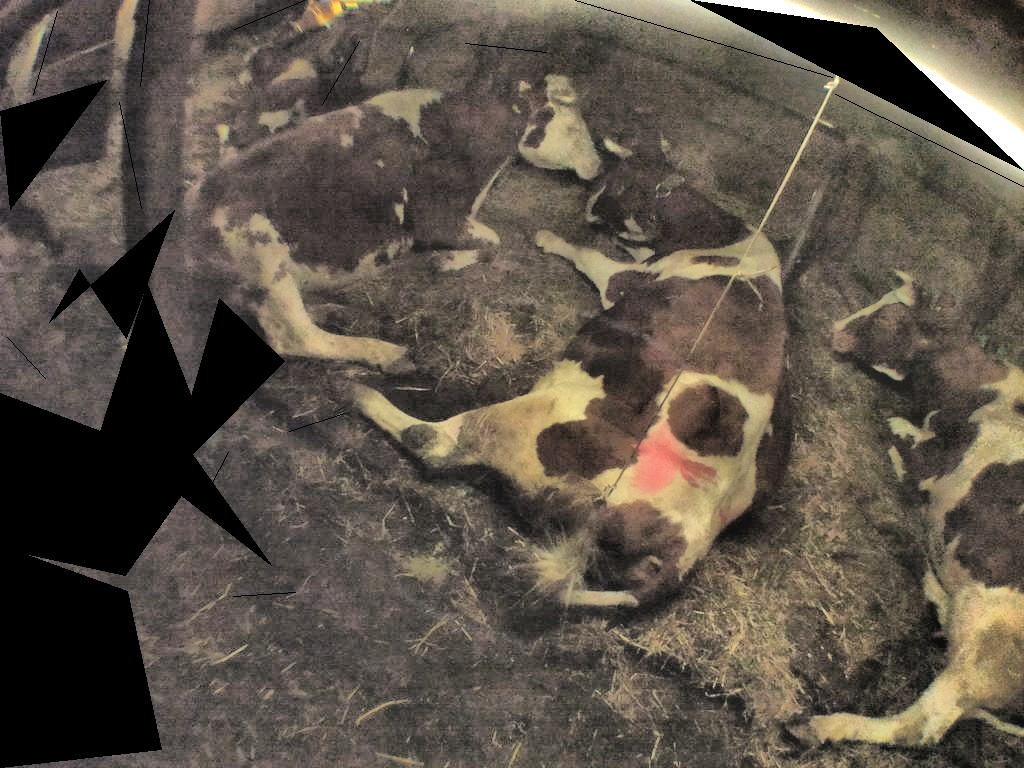
\includegraphics[scale=0.43]{Grafiken/entwicklung/7unwichtigePolygone.jpg}
	\caption{Unwichtige Bereiche als Polygone } 
	\label{fig: Unwichtige Bereiche als Polygone}
\end{figure}

Weiter wurde versucht, die unwichtige Fläche im Originalbild durch konvexe Hüllen zu maximieren. Das Bild \ref{fig: Unwichtige Bereiche als konvexe Hülle} zeigt konvexe Hüllen der Konturen,  die als Ergebnisse der Funktion \texttt{convexHull()} entstehen.

\begin{figure}[H]
	\center
	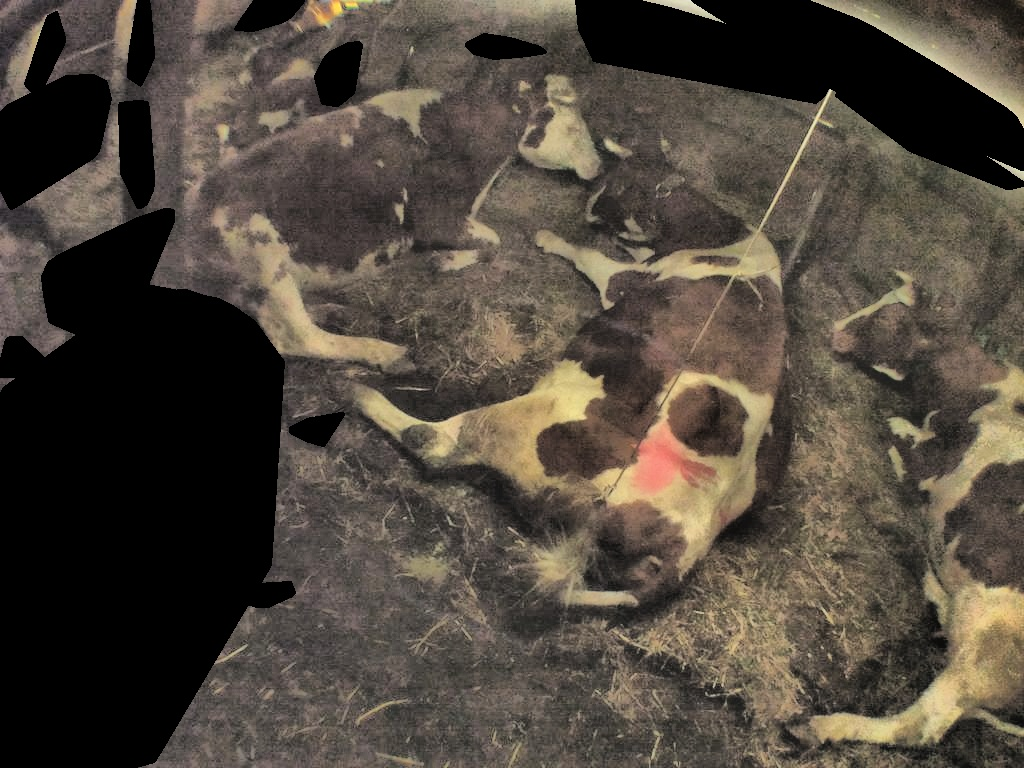
\includegraphics[scale=0.43]{Grafiken/entwicklung/7unwichtigeKonvexe.jpg}
	\caption{Unwichtige Bereiche als konvexe Hülle} 
	\label{fig: Unwichtige Bereiche als konvexe Hülle}
\end{figure}

 Als weiterer Lösungsansatz wurde die Funktion \texttt{minEnclosingCircle()} verwendet, um Kreise zu finden, welche Konturen mit möglichst geringer Fläche umschliessen (Abbildung \ref{fig: Unwichtige Bereiche als Kreise}).
 
\begin{figure}[H]
	\center
	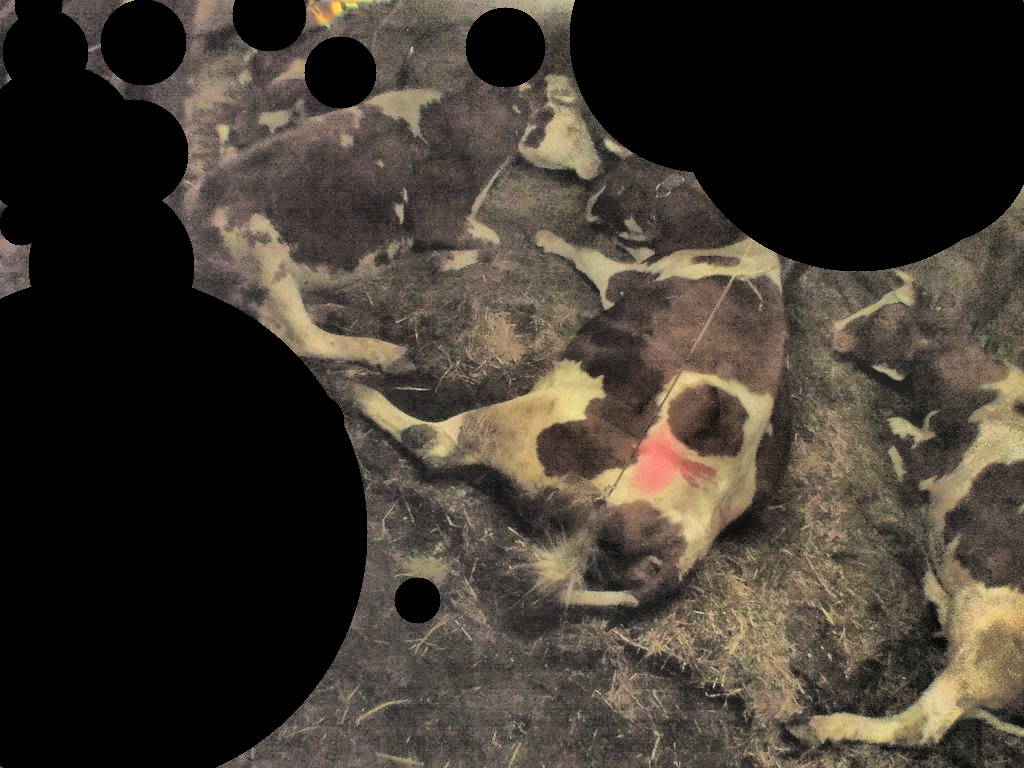
\includegraphics[scale=0.43]{Grafiken/entwicklung/7unwichtigeKreise.jpg}
	\caption{Unwichtige Bereiche als Kreise } 
	\label{fig: Unwichtige Bereiche als Kreise}
\end{figure}
Abschliessend wurden für die Abbildung \ref{fig: Unwichtige Bereiche als Rechtecke} mit der Funktion \texttt{boundingRect()} Rechtecke gebildet, welche die Konturen umschliessen.
\begin{figure}[H]
	\center
	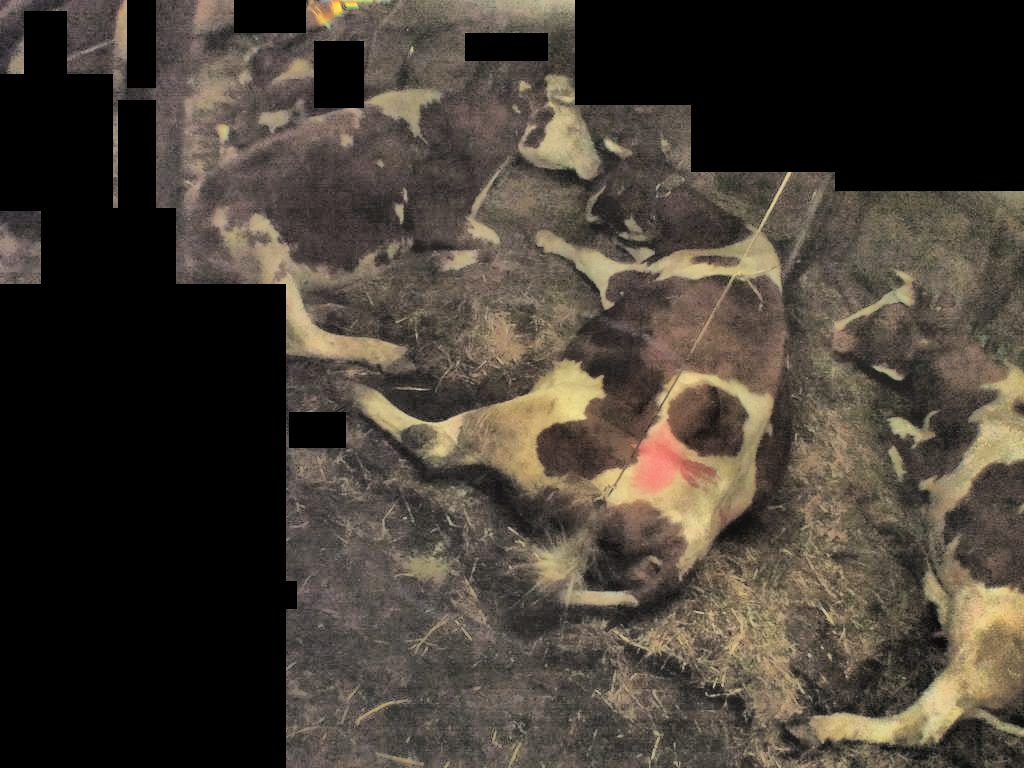
\includegraphics[scale=0.43]{Grafiken/entwicklung/7unwichtigeRechtecke.jpg}
	\caption{Unwichtige Bereiche als Rechtecke} 
	\label{fig: Unwichtige Bereiche als Rechtecke}
\end{figure}


Die Verfahren, welche mittels \texttt{minEnclosingCircle()} und \texttt{boundingRect()} angewendet werden, ergeben im vorliegenden Kontext die besten Ergebnisse. Einerseits werden die als unwichtig identifizierten Flächen  maximiert. Andererseits werden nur sehr kleine Bereiche der Kuh fälschlicherweise als unwichtig eingestuft. Da perfekte Kreise in nach der Ermittlung der Konturen mihilfe von \texttt{findContours()} bei den Kühen nicht vorkommen, entscheidet sich der Autor dafür, unwichtige Bereiche als schwarze Kreise einzuzeichnen. Zudem können diese Kreise in der weiteren Bildbearbeitung problemlos als solche erkannt werden.
Dementsprechend wird das in Abbildung \ref{fig: Unwichtige Bereiche als Kreise} dargestellte Bild zur weiteren Analyse verwendet.
An dieser Stelle ist jedoch auch Kritik an dieser Methode zur Bestimmung von unwichtigen Bereichen angebracht. Die Funktion \texttt{inRange()} benötigt einen Wertebereich für Farben, um die unwichtigen Bereiche zu finden. Dieser Wertebereich ist stark von den Lichtverhältnissen im untersuchten Bild abhängig. Bei Tests mit verschiedenen Bildern, die ebenfafalls mit dem Rasperry Pi aufgenommen wurden, haben hat die falsche Detektierung von unwichtigen Bereichen das Gesamtergebnis verschlechtert. Aus diesem Grund wird mittels Konfiguration \texttt{AdvancedUnimportantColorRange=False} die Möglichkeit geboten, nur die Farbbereiche der Lampe zu nutzen. Diese wird in allen durchgeführten Tests zuverlässig detektiert.  
\subsection{Detektierung von wichtigen Bereichen im Bild}



In einem ersten Schritt wird die geglättete und aufgehellte Version von Bild \ref{fig: Unwichtige Bereiche als Kreise} mit dem adaptiven Schwellwertverfahren bearbeitet. Um dies zu erreichen, wird die Funktion \texttt{adaptiveThreshold()} mit den Argumenten \texttt{THRESH_BINARY_INV} und \texttt{ADAPTIVE_THRESH_MEAN_C} aufgerufen. Das Ergebnis dieses Versuchs, wichtige Bereiche des Bilds zu detektieren, ist in Abbildung \ref{fig: Detektierung von wichtigen Bereichen mittels adaptivem Schwellwertverfahren} ersichtlich. Die angestrebte Partitionierung des Bildes in Bereiche der Kuh und in alle anderen Bereiche funktioniert nicht. Deshalb wird der Versuch mit denselben Einstellungen aber mit einem nicht geglätteten Bild wiederholt.

\begin{figure}[H]
	\center
	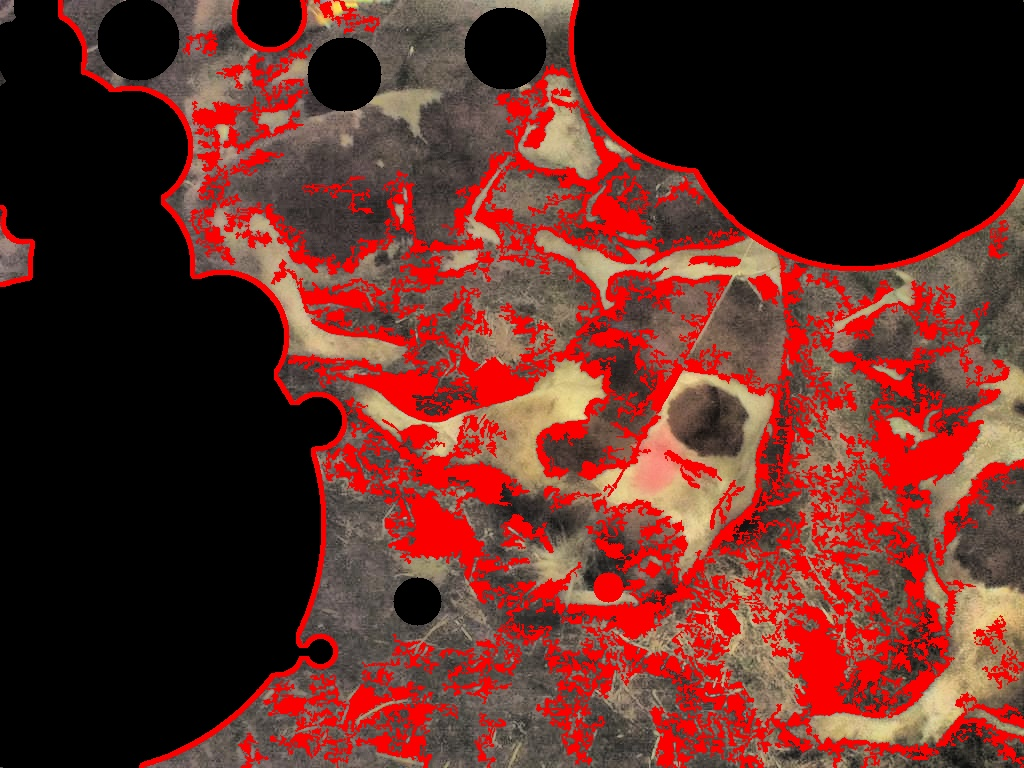
\includegraphics[scale=0.43]{Grafiken/entwicklung/10thresholdedEqualizedBirghtened.jpg}
	\caption{Detektierung von wichtigen Bereichen mittels adaptivem Schwellwertverfahren} 
	\label{fig: Detektierung von wichtigen Bereichen mittels adaptivem Schwellwertverfahren} 
\end{figure}

Das Ergebnis ist in Abbildung \ref{fig: Versuch, aus nicht geglättetem Bild wichtige Bereiche zu detektieren} dargestellt und stellt ein besseres Zwischenergebnis dar. Als entsprechende Erkenntnis leitet der Autor ab, dass die Glättung von Histogrammen zwar die Bildqualität und Interpretationsfähigkeit für den Menschen steigert, aber im vorliegenden Kontext auch negativen Einfluss auf das Schwellwertverfahren hat.

\begin{figure}[H]
	\center
	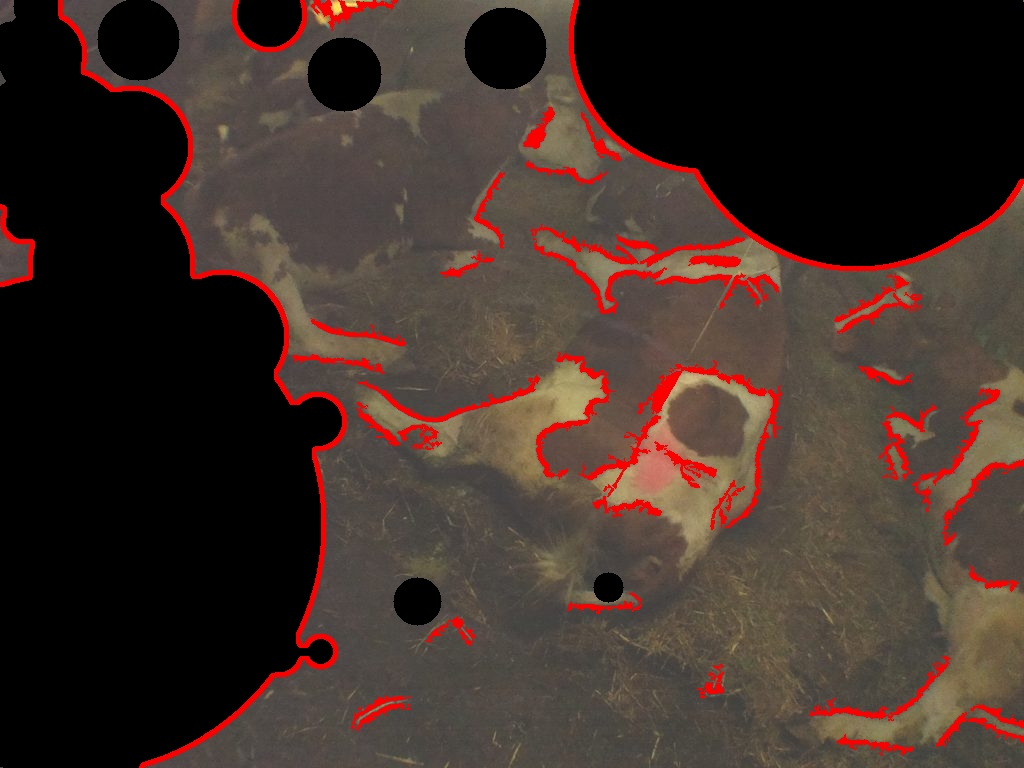
\includegraphics[scale=0.43]{Grafiken/entwicklung/11thresholdedNotEqualized.jpg}
	\caption{Versuch, aus nicht geglättetem Bild wichtige Bereiche zu detektieren} 
	\label{fig: Versuch, aus nicht geglättetem Bild wichtige Bereiche zu detektieren} 
\end{figure}

Abbildung \ref{fig: Versuch, aus nicht geglättetem Bild wichtige Bereiche zu detektieren} zeigt das Resultat einer vielversprechenden Analyse. Das Ergebnis ist aber insofern kritisch zu beurteilen, da die rote Farbe die gesamte Kontur ausfüllt, die detektiert wurde. Dementsprechend werden die Beine beispielsweise nicht als Kontur erkannt, sondern lediglich die Umrisse davon.
Dies dient als Motivation, die Konfiguration des Schwellwertverfahren anzupassen. Demzufolge wurde mit der Funktion \texttt{threshold()} und den Argumenten \texttt{THRESH_BINARY} als Verfahrenstyp, und dem Wert \texttt{90} als Schwellwert angewendet. Das Ergebnis daraus ist in Abbildung \ref{fig: Ergebnisse nach angepasster Konfiguration des Schwellwertverfahrens} dargestellt. Die als unwichtig identifizierten Bereiche werden nicht mehr berücksichtigt.
\begin{figure}[H]
	\center
	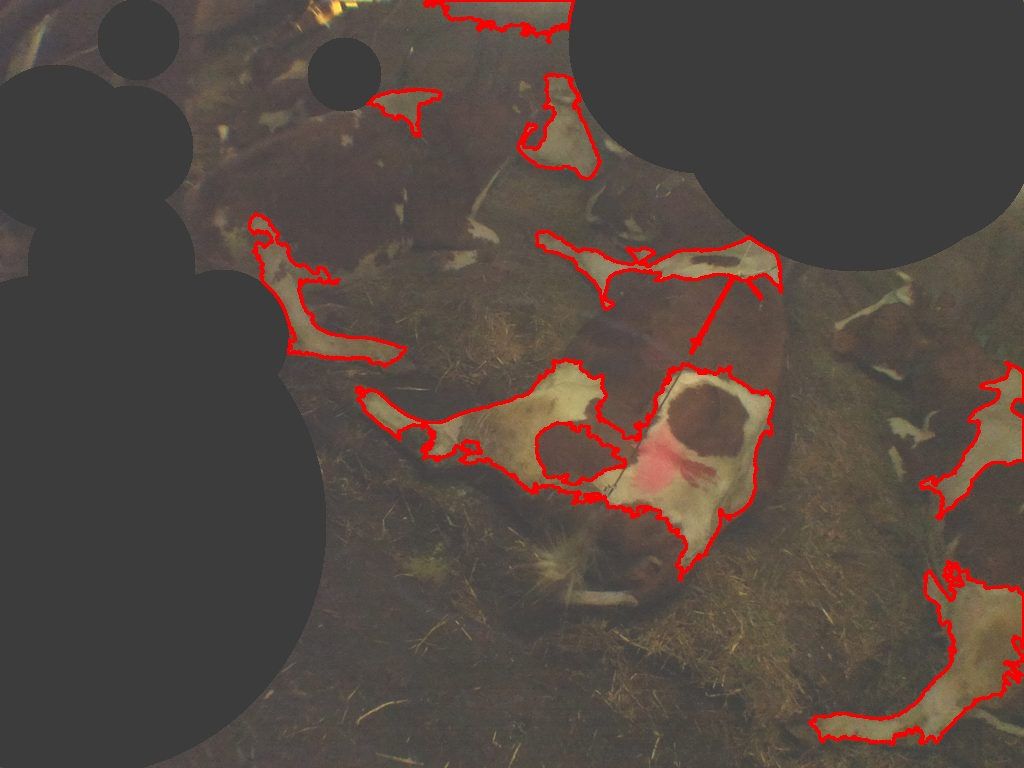
\includegraphics[scale=0.43]{Grafiken/entwicklung/12SimpleThresholdingConoturOutlineCCOMP.jpg}
	\caption{Ergebnisse nach angepasster Konfiguration des Schwellwertverfahrens} 
	\label{fig: Ergebnisse nach angepasster Konfiguration des Schwellwertverfahrens} 
\end{figure}
Es fällt nun auf, dass Flecken innerhalb der Kontur der Kuh erkannt werden. Da \texttt{findContours()} mit dem Argument \texttt{RETR_CCOMP} aufgerufen wird, werden auch Konturen innerhalb von den äusseren Konturen zurückgegeben und in eine  Hierarchie eingeteilt. Die äusseren Konturen entsprechen in den meisten Fällen den Umrissen der Kuh oder der Flecken. Zum aktuellen Zeitpunkt reicht es aus, nur diese Umrisse zu erkennen und dementsprechend wird \texttt{findContours()} mit dem Argument \texttt{RETR_EXTERNAL} aufgerufen. Das Ergebnis ist in Abbildung  \ref{fig: Ergebnisse nach angepasster Konfiguration des Contour Finders} sichtbar.
\begin{figure}[H]
	\center
	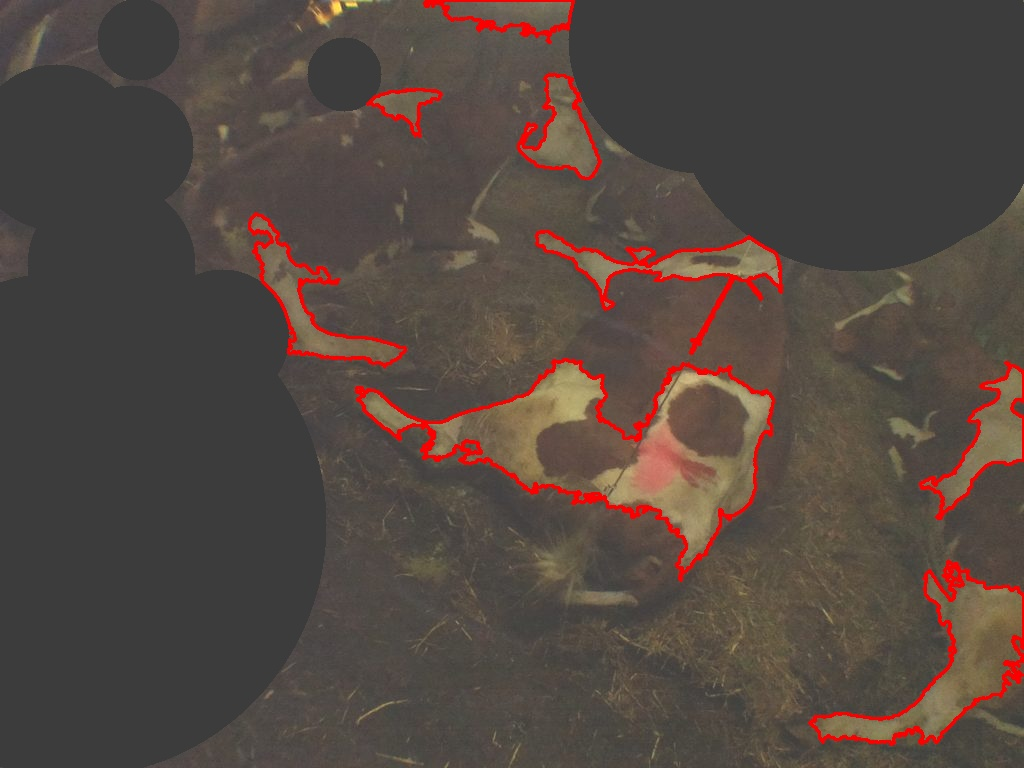
\includegraphics[scale=0.43]{Grafiken/entwicklung/13SimpleThresholdingConoturOutlineLIST.jpg}
	\caption{Ergebnisse nach angepasster Konfiguration des Contour Finders} 
	\label{fig: Ergebnisse nach angepasster Konfiguration des Contour Finders} 
\end{figure}

Dabei unterscheiden sich die Ergebnisse bei der Anwendung von \texttt{findContours()} mit unterschiedlichen Approximationsverfahren wie \texttt{CHAIN_APPROX_SIMPLE}, \texttt{CHAIN_APPROX_TC89_L1}, \texttt{CHAIN_APPROX_TC89_KCOS} von der Deaktivierung der Approximation  nicht wesentlich.

Da nun lediglich äussere Konturen detektiert werden, dürfen diese Konturen mit Farbe gefüllt werden, ohne relevante Informationen über Hierarchien zu vernichten (Abbildung \ref{fig: Konturen mit Farbe gefüllt}).

\begin{figure}[H]
	\center
	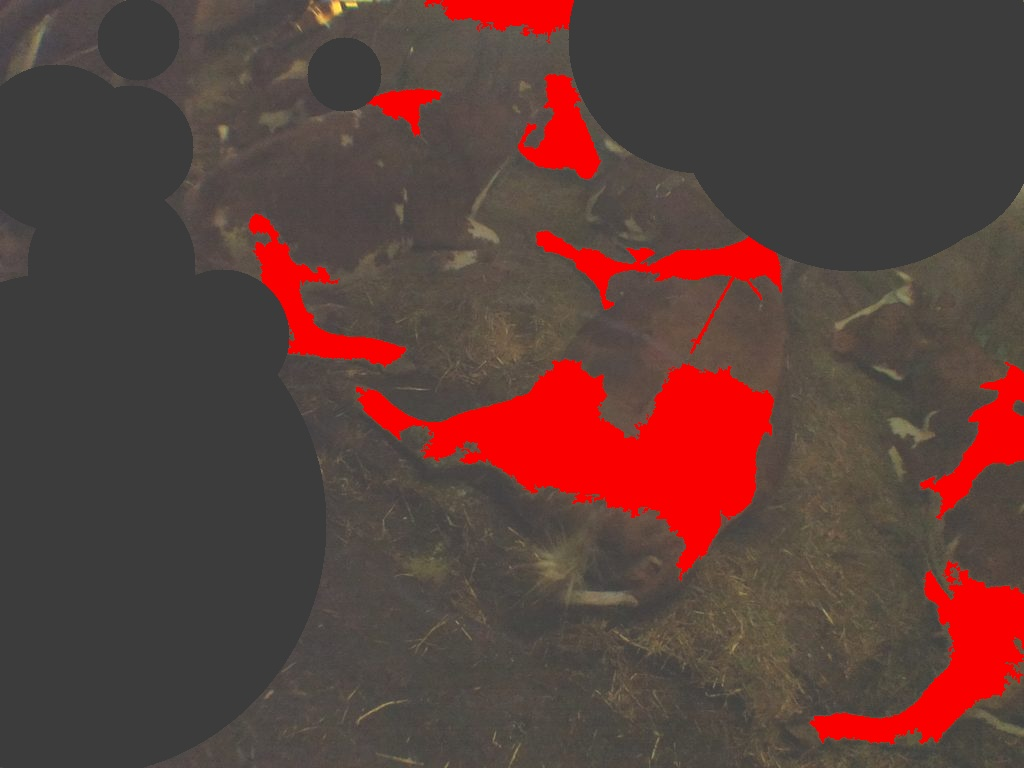
\includegraphics[scale=0.43]{Grafiken/entwicklung/14AfterThresholdingContourFilled.jpg}
	\caption{Konturen mit Farbe gefüllt} 
	\label{fig: Konturen mit Farbe gefüllt} 
\end{figure}


\subsection{Erkennung von seitlich liegender Kuh}
Aus der Domänenanalyse und Experteninterviews hat sicher ergeben, dass seitliches Liegen ein starkes Geburtsanzeichen ist und entsprechend detektiert werden muss. Die Seitenlage charakterisiert sich unter anderem mit gestreckten Beinen. Um diese zu erkennen, werden die geometrischen Eigenschaften der detektierten Konturen nachfolgend mit unterschiedlichen Verfahren analysiert. Diese Analyse soll die Filterung der unwichtigen Konturen erlauben. 

 Da nun keine weiteren Konturen mehr gesucht werden (kein Aufruf von \texttt{findContours()}), sind nachfolgend sämtliche dargestellten Bilder bearbeitet, um deren Helligkeit und Kontrast zu erhöhen. Dies wurde unter Anwendung der Funktionen \texttt{add()} und \texttt{createCLAHE()} gemacht. Zudem wurden die schwarze Kreise, welche unwichtige Bereiche des Bildes verdecken entfernt. Dies erhöht die Lesbarkeit des Berichts. Zudem wurden Rechtecke gezeichnet, welche die Konturen jeweils umschliessen. Diese Erhöhen das Verständnis von den geometrischen Eigenschaften und Filterungen. Dabei werden Konturen, als Resultat der Analyse als wichtig befunden wird jeweils rot eingefärbt. Diese werden schrittweise gefiltert. Konturen, welche in einem Zwischenschritt als unwichtig erkannt werden, werden mit grüner Farbe gefüllt. 

\begin{figure}[H]
	\center
	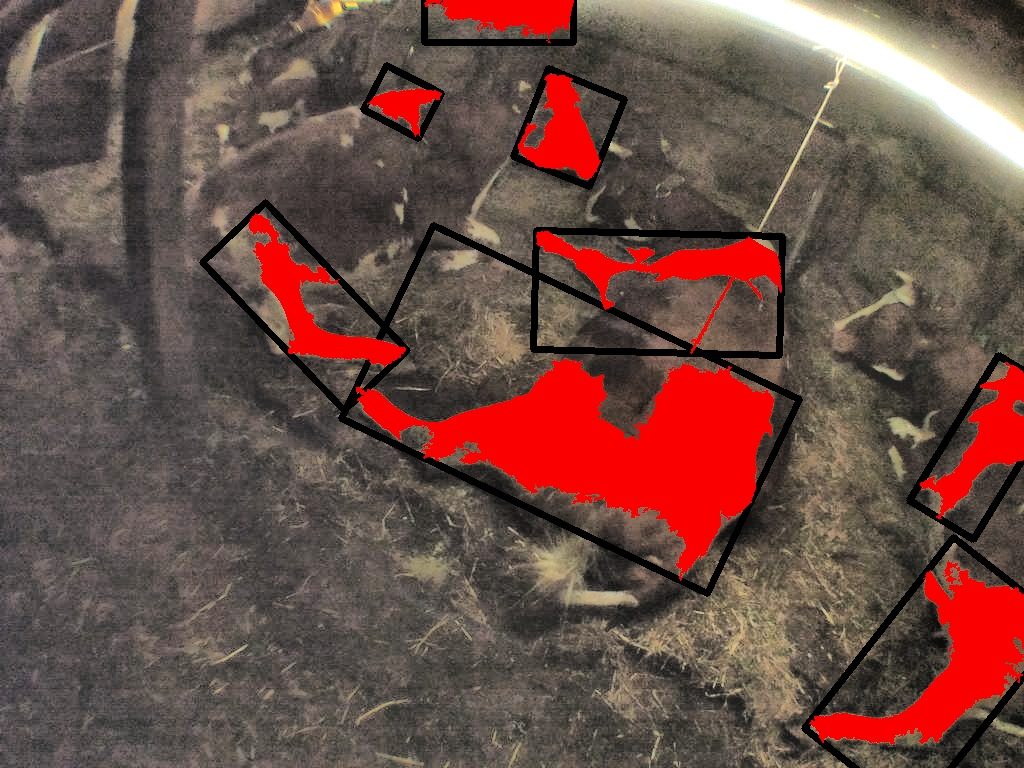
\includegraphics[scale=.43]{Grafiken/entwicklung/20StartImage.jpg}
	\caption{Ausgangslage vor der Analyse und Filterung der Konturen} 
	\label{fig: Ausgangslage vor der Analyse und Filterung der Konturen} 
\end{figure}

\subsubsection{Filterung der Konturen nach Winkel}
Typischerweise strecken Kühe in Seitenlage die Beine ungefähr rechtwinklig vom Körper weg. Die Infrastruktur vom Bauernhof des Arbeitgebers im Schwellibach ist auf Anbindehaltung ausgelegt. Wenn der Stall voll ist, also in jeder Box eine Kuh ist, liegen die Kühe beim Kalbern gerade in der Box \citep{Muller2020b}. Dementsprechend können Konturen als unwichtig betrachtet werden, wenn deren Ausrichtung stark von 90$^{\circ}$  abweicht. Als Referenzobjekt für die Messung des Winkels dient die Lampe, welche in Realität rechtwinklig zur Box der Kuh und waagrecht montiert ist. Da die Lampe in Bildern nicht waagrecht abgebildet ist, werden die Winkel sämtlicher Konturen um diese Abweichung bereinigt (Formel \ref{Bereinigung der Winkel}). Für die Messung der Winkel wurde die Funktion \texttt{fitEllipse()} verwendet, welche den Winkel der entsprechenden Ellipse zurückgibt.

\begin{equation}\label{Bereinigung der Winkel}
\delta_{i} = (\alpha_{i} - \beta + \gamma) \bmod 360
\end{equation}

wobei $ \delta_{i} $ dem bereinigten Winkel von Kontur ${i}$,  $ \alpha_{i} $ dem gemessener Winkel von Kontur ${i}$, $\beta$ dem tatsächlichen Winkel der Lampe und $\gamma$ dem erwarteten Winkel der Lampe entspricht.


Das Vorgehen gleicht grundsätzlich dem Prinzip, das Bild solange zu drehen, bis die Lampe waagrecht im Bild ist und erst dann die Winkel zu messen. Abbildung \ref{fig: Veranschaulichung zur Analyse der Winkel} veranschaulicht die Überlegung. 


\begin{figure}[H]
	\center
	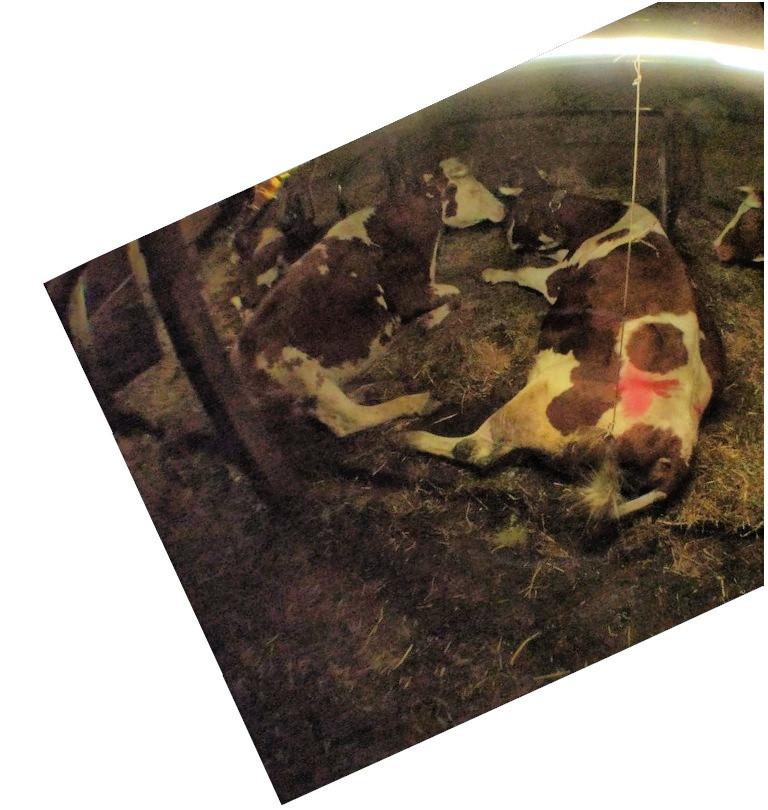
\includegraphics[scale=1.3]{Grafiken/entwicklung/21AngleCorrecturDemonstration.jpg}
	\caption{Veranschaulichung zur Analyse der Winkel} 
	\label{fig: Veranschaulichung zur Analyse der Winkel} 
\end{figure}


Die Abbildung \ref{fig: Ergebnisse nach Filterung der Konturen nach Winkel} zeigt in roter Farbe die Konturen, welche weiterhin als Beine von seitlich liegenden Kühen vermutet werden und entsprechend weiter analysiert werden. Die bereinigten Winkel der grün eingefärbten Konturen liegen nicht im Wertebereich zwischen \texttt{70-}\texttt{110}$^{\circ}$. Dabei sind die maximalen und minimalen Werte der betrachteten Winkel in der entwickelten Lösung mittels \texttt{MIN_LEG_ANGLE_EXPECTION} und \texttt{MAX_LEG_ANGLE_EXPECTION} konfigurierbar. 
\begin{figure}[H]
	\center
	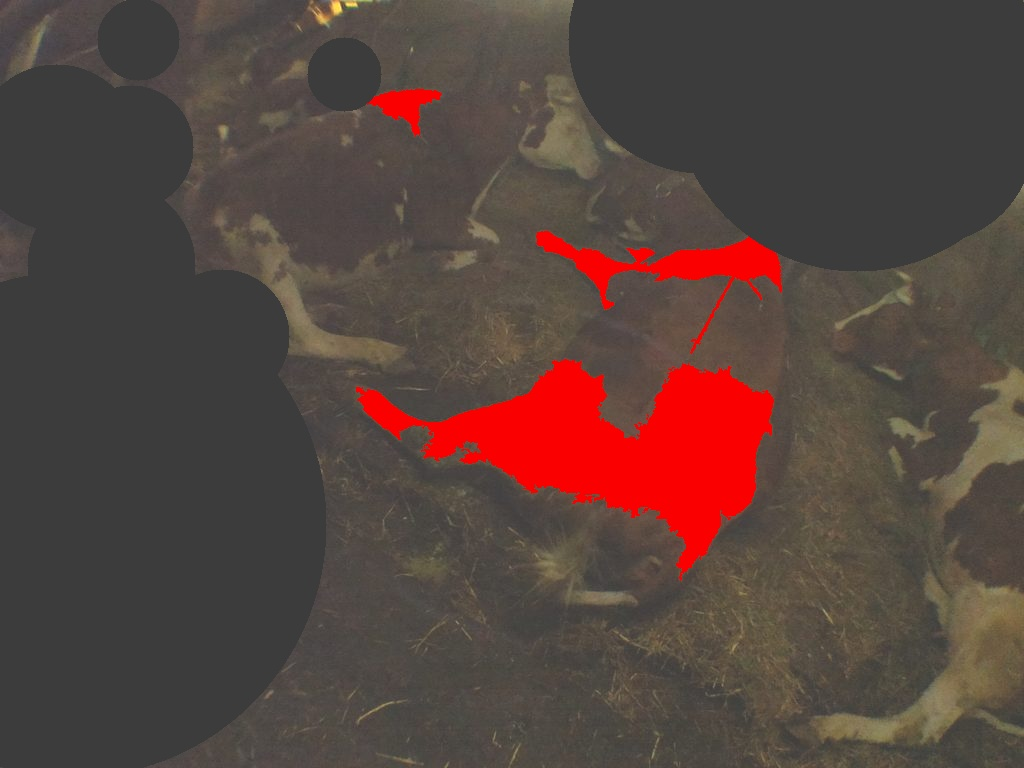
\includegraphics[scale=0.43]{Grafiken/entwicklung/22AngleCorrectur.jpg}
	\caption{Ergebnisse nach Filterung der Konturen nach Winkel} 
	\label{fig: Ergebnisse nach Filterung der Konturen nach Winkel} 
\end{figure}

Eine Ausnahme stellt ein nicht voller Stall dar. Leere Boxen ermöglichen der kalbernden Kuh, quer in die Box zu liegen \citep{Muller2020b}. Für Kühe, welche neben einer leeren Box liegen, ist also die Filterung der Konturen nach Winkel nicht sinnvoll. Um dieser Situation gerecht zu werden, kann im entwickelten System mittels Konfiguration \texttt{filterbyAngle=False} die Filterung nach Winkel deaktiviert werden. 


\subsubsection{Filterung der Konturen nach Extent}
Um diese Ergebnisse weiter zu analysieren, wurde mittels \texttt{minAreaRect()} für jede Kontur das Rechteck ermittelt, welches mit der kleinsten Fläche sämtliche Punkte der Kontur einschliesst. Die Rechtecke wurden schwarz ins Originalbild eingezeichnet. 
Dies dient als Grundlage des \flqq Extent\frqq. Dabei handelt es sich um das Verhältnis zwischen der Fläche der Kontur und der Fläche des Rechtecks, das die Kontur einschliesst (Formel \ref{Extent}).

\begin{equation}\label{Extent}
Extent =  \frac{Fl\ddot{a}che\ der\ Kontur}{Fl\ddot{a}che\  umschliessendes\  Rechteck}  
\end{equation}

Der Autor erwartet, dass die Fläche der Kontur der Beine gegenüber dem darum gebildeten Rechteck klein ist. Entsprechend wird für als Extent bei Beinen ein tiefer Wert angenommen im Vergleich zum Wert des Extent bei anderen Figuren. Dementsprechend ermöglicht die entwickelte Lösung die Konstante \texttt{EXTENT_MAX} die Konfiguration eines Schwellwerts, nach welchem Konturen gefiltert werden. 

Nun wird als Schwellwert für Extent \texttt{0.5} angenommen und entsprechend werden nur noch Konturen berücksichtigt, welche unterhalb dieses Werts liegen. In Abbildung \ref{fig: Ergebnis der Filterung der Konturen nach Extent} sind alle Konturen mit ${Extent < 0.5}$ rot und alle anderen Konturen grün eingefärbt. Das Ergebnis ist positiv, zwei unerwünschte Konturen können als solche erkannt werden.
\begin{figure}[H]
	\center
	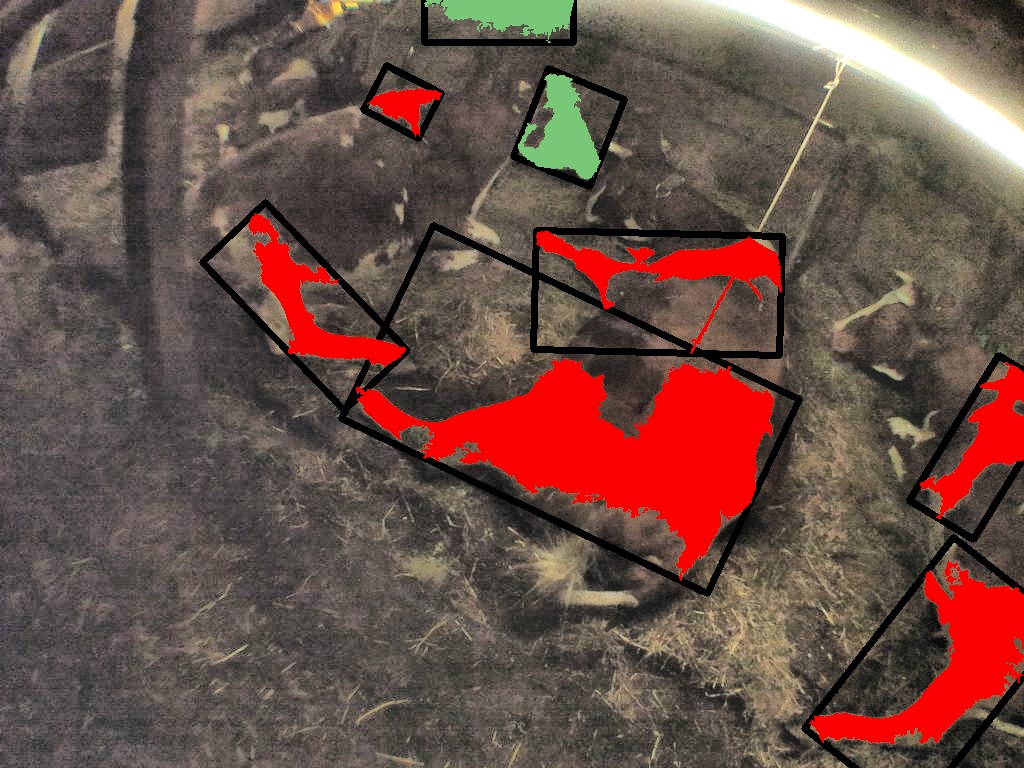
\includegraphics[scale=0.43]{Grafiken/entwicklung/23FilteringExtent.jpg}
	\caption{Ergebnis der Filterung der Konturen nach Extent } 
	\label{fig: Ergebnis der Filterung der Konturen nach Extent} 
\end{figure}

Abbildung \ref{fig: Ergebnis der Filterung der Konturen nach Winkel und Extent } veranschaulicht die Kombination der Filterung nach Winkel und Extent. Es können erfolgreich unwichtige Konturen gefiltert werden. Um die Ergebnisse der Analyse zu verbessern, sind jedoch zusätzlich Filterungen nötig.
\begin{figure}[H]
	\center
	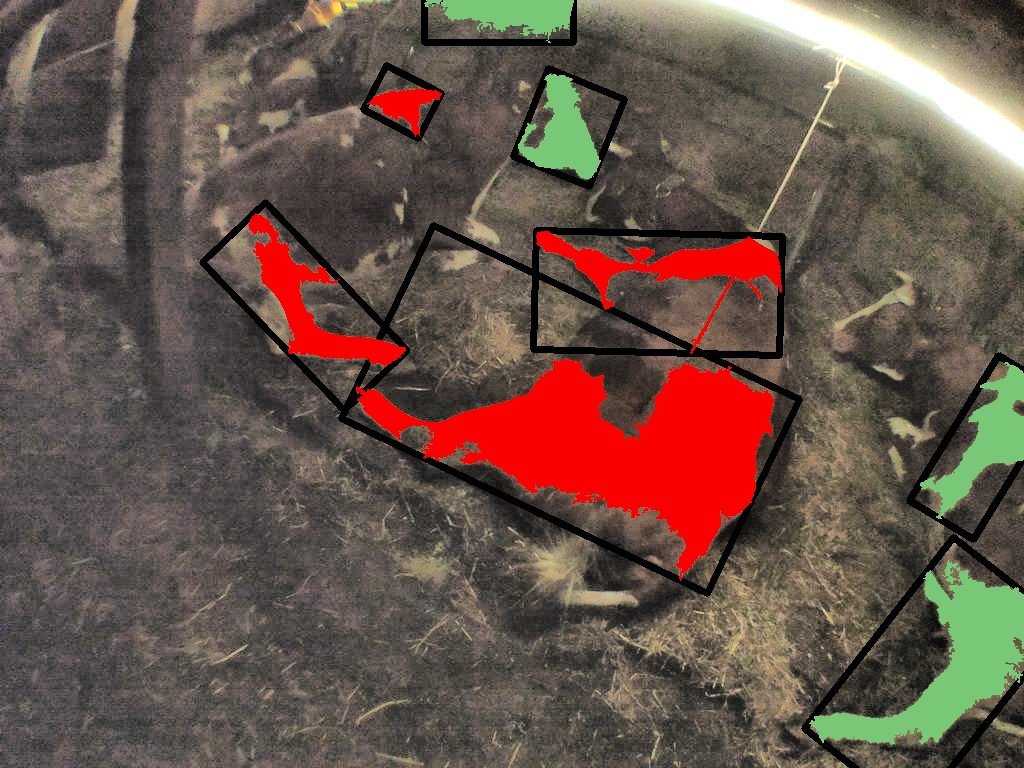
\includegraphics[scale=0.43]{Grafiken/entwicklung/24FilteringExtentAngle.jpg}
	\caption{Ergebnis der Filterung der Konturen nach Winkel und Extent  } 
	\label{fig: Ergebnis der Filterung der Konturen nach Winkel und Extent } 
\end{figure}

\subsubsection{Filterung der Konturen nach Aspect Ratio}

Rechtecke, welche die Beine der Kuh einschliessen, sind langgezogen. Der Autor überprüft nun die Vermutung, dass diese Eigenschaft dabei hilf, Beine von unwichtigen Konturen zu unterscheiden. Das Verhältnis zwischen Breite und Höhe von Rechtecken (nachfolgend Aspect Ratio genannt) liefert Informationen darüber, wie langgezogen ein Rechteck ist.	
	
\begin{equation}\label{Aspect Ratio}
Aspect\ Ratio =  \frac{Breite}{H\ddot{}he}  
\end{equation}
Da für den Autor grundsätzlich nicht das Verhältnis zwischen Breite und Höhe sondern das Verhältnis zwischen der langen und der kurzen Seite des Rechtecks entscheidend ist, wird die Formel \ref{Aspect Ratio} aus angepasst. Formel \ref{Angepasste Aspect Ratio} beschreibt, was in der technischen Implementierung realisiert wird.
\begin{equation}\label{Angepasste Aspect Ratio}
Aspect\ Ratio =  \frac{lange \ Seite}{kurze \ Seite}  
\end{equation}

Das Ergebnis der Filterung von Konturen mit dem Schwellwert \texttt{1.5} ist in Abbildung \ref{fig: Ergebnis der Filterung von Konturen nach Aspect Ratio} abgebildet. Die Filterung der Konturen kann dadurch verbessert werden.
\begin{figure}[H]
	\center
	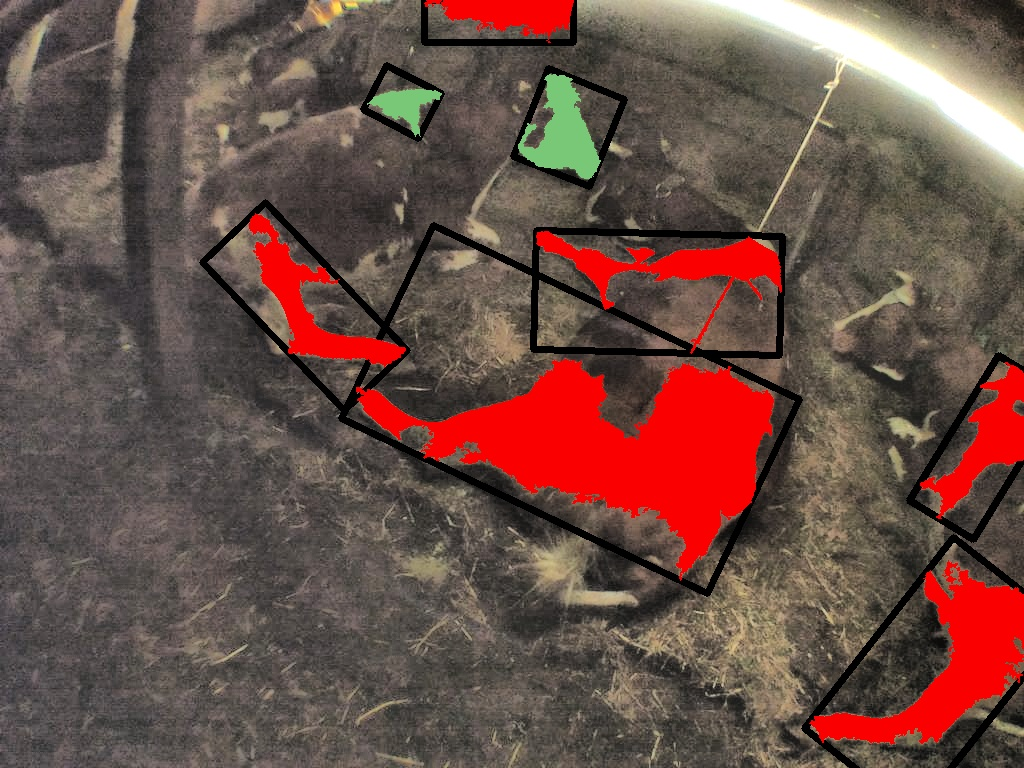
\includegraphics[scale=0.43]{Grafiken/entwicklung/27AspectRatio.jpg}
	\caption{Ergebnis der Filterung von Konturen nach Aspect Ratio } 
	\label{fig: Ergebnis der Filterung von Konturen nach Aspect Ratio} 
\end{figure}
\subsubsection{Kombination der Filter nach Winkel, Extent und Aspect Ratio }
Durch Kombination der Filterung nach Winkel, Extent und Aspect Ratio, erreicht man das Resultat gemäss Abbildung \ref{fig: Ergebnis der Filterung der Konturen nach Winkel, Extent und Aspect Ratio}. Dabei werden Konturen mit einem bereinigten Winkel zwischen \texttt{70} und \texttt{110}$^{\circ}$, Extent unter 0.5 und Aspect Ratio über 1.5 berücksichtigt.



\begin{figure}[H]
	\center
	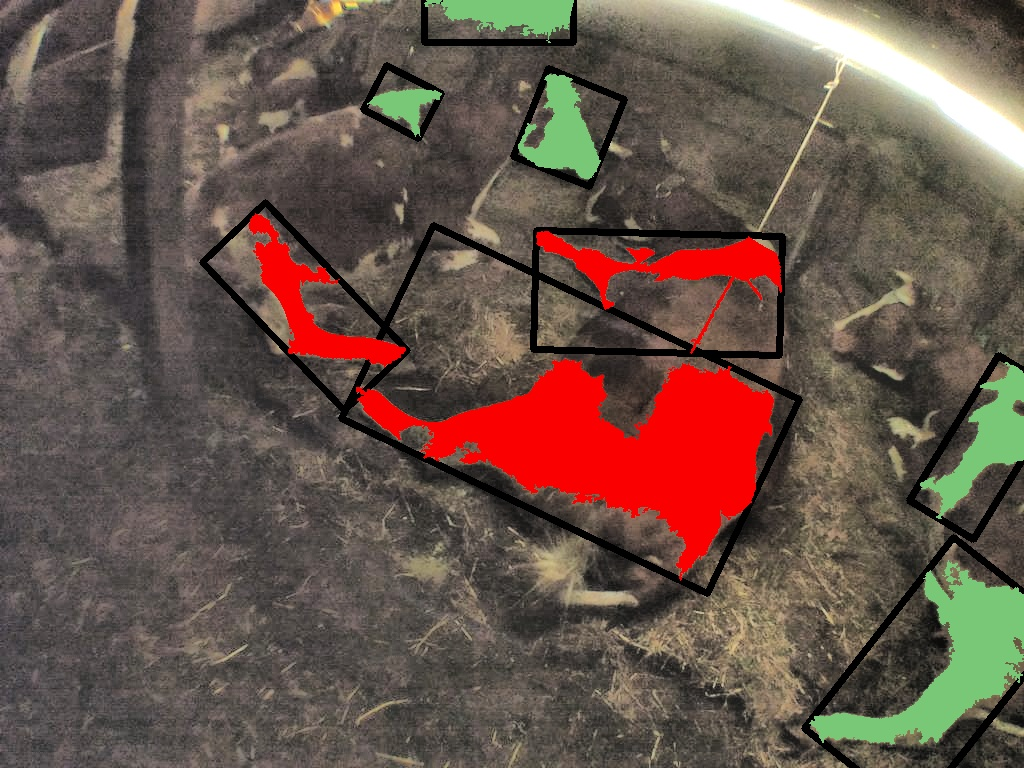
\includegraphics[scale=0.43]{Grafiken/entwicklung/30FilteredByExtentAspectAngle.jpg}
	\caption{Ergebnis der Filterung der Konturen nach Winkel, Extent und Aspect Ratio} 
	\label{fig: Ergebnis der Filterung der Konturen nach Winkel, Extent und Aspect Ratio} 
\end{figure}

\subsubsection{Filterung mittels Shape Matching }
Nun werden vier Konturen als potentielle Konturen von Beinen bei seitlichem Liegen erkannt. Wünschenswert wäre nun, diese Auswahl weiter einzugrenzen. Um dies zu erreichen, sind Unterschiede der Konturen von den Beinen der mittleren Kuh und der Kontur des Hinterbeins der linken Kuh zu ermitteln. In erster Linie hat der Autor versucht, die Orientierung der Beine zu erkennen. Beim seitlichen Liegen der Kuh zeigen zwei Beine in dieselbe Richtung und deren Abstand liegt innerhalb eines bestimmten Bereichs. Anhand der Ausrichtung der Beine kann mit den bereits angewendeten Funktionen \texttt{minAreaRect()} und \texttt{fitEllipse()} keine weitere Filterung etabliert werden. Der Grund dafür ist, dass sämtliche Winkel in einem sehr ähnlichen Wertebereich sind. Auch die Messung des Abstands zwischen den Beinen stellt ist mit den bereits angewendeten Mitteln nicht möglich. Der Autor ist der Meinung, dass sich im betrachteten Bild in erster Linie der Holzträger als Referenzobjekt für die Messung von Distanzen eignet. Dieser ist jedoch nicht in voller Länge im Bild, was die Messung ungenau macht. Darüber hinaus ist dieser Holzträger nicht in jedem Bild an derselben Stelle und auch nicht in jedem Bild sichtbar. Die Konturen der Beine sind keine geeigneten Referenzobjekte, da diese gestreckt oder gebeugt sein können. Der Autor ist der Ansicht, dass ein Referenzobjekt im Bild platziert werden müsste, um gute Resultate zu erreichen. Dieses Referenzobjekte sollte durch Methoden der Bildanalyse eindeutig zu erkennen sein.

An dieser Stelle verfolgt der Autor einen anderen Lösungsansatz. Die Funktion \texttt{matchShapes()} vergleicht sämtliche verbleibende Konturen und gibt eine Metrik zurück, welche die Ähnlichkeit der Konturen repräsentiert. Die Funktion unterstützt die drei Modi \texttt{CONTOURS_MATCH_I1}, \texttt{CONTOURS_MATCH_I2} und \texttt{CONTOURS_MATCH_I3} \citep[S. 392]{FernandezVillan2019}. Sämtliche Modi ergeben im vorliegenden Kontext keinen Beitrag zur weiteren Filterung der Konturen. Bild \ref{fig: Ergebnis der Shape Matching}) zeigt die Anwendung von \texttt{matchShapes()} mit dem Modus \texttt{CONTOURS_MATCH_I1} und dem Schwellwert \texttt{5}. Die Konturen der Hinterbeine der zwei Kühe werden als ähnlicher betrachtet als die Konturen der Beine derselben Kuh. 

\begin{figure}[H]
	\center
	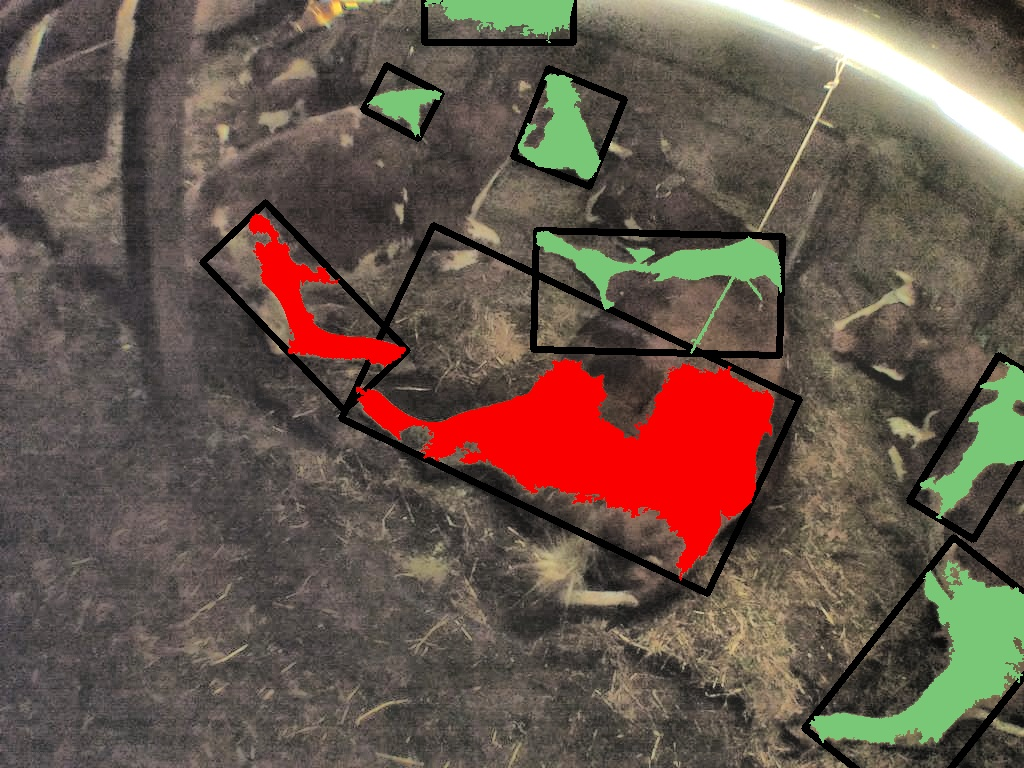
\includegraphics[scale=0.43]{Grafiken/entwicklung/31FilteredBySimilarity.jpg}
	\caption{Ergebnis der Shape Matching} 
	\label{fig: Ergebnis der Shape Matching} 
\end{figure}
Im angewandten Verfahren der Bildanalyse wurden die Winkel der Konturen bereits berücksichtigt. Um sicherzustellen, dass das Resultat von \texttt{matchShapes()} nicht auf die Winkel der Konturen zurückzuführen ist, werden sämtliche verbleibende Konturen auf einen zufällig ausgewählten Winkel von 60$^{\circ}$ verschoben. Anschliessend werden die Konturen wieder mit \texttt{matchShapes()} verglichen. Das Ergebnis ist dasselbe, die Klassifikation kann zu diesem Zeitpunkt nicht weiter verbessert werden. Abbildung \ref{fig: Ergebnis der Shape Matching und Korrektur der Winkel} zeigt die das Ergebnis der verschobenen Konturen mit einem weissen Hintergrund.
\begin{figure}[H]
	\center
	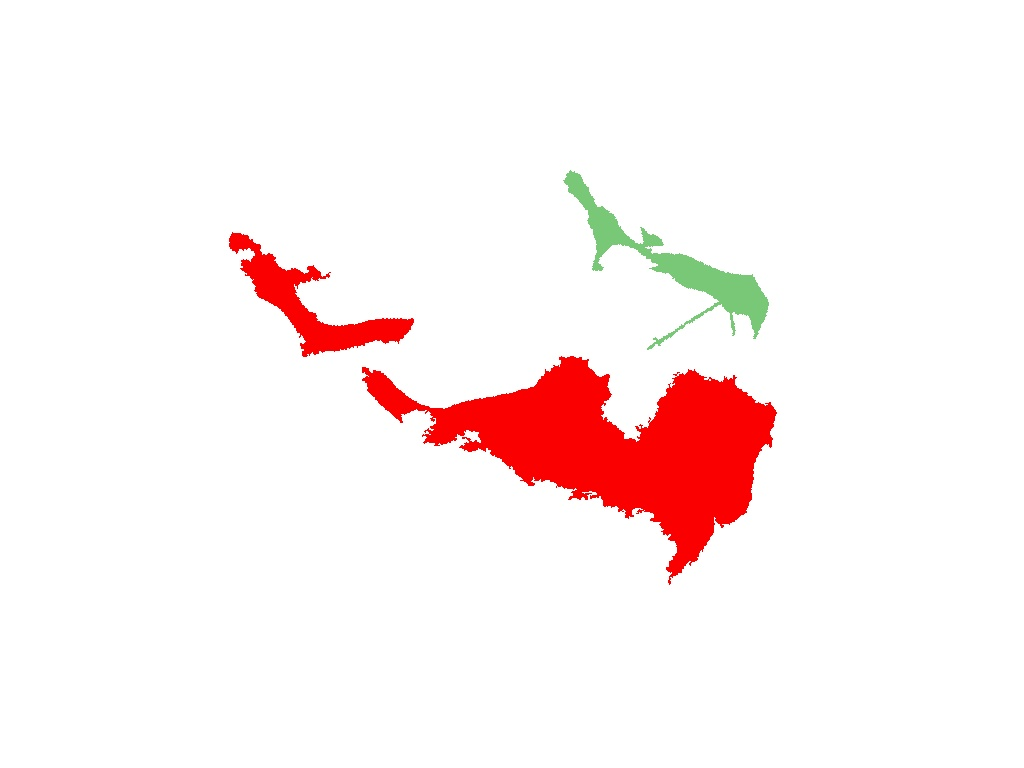
\includegraphics[scale=0.43]{Grafiken/entwicklung/32BlankFilteredBySimilarity.jpg}
	\caption{Ergebnis der Shape Matching und Korrektur der Winkel} 
	\label{fig: Ergebnis der Shape Matching und Korrektur der Winkel} 
\end{figure}


Die Abbildung \ref{fig: Ergebnis der Filterung der Konturen nach Winkel, Extent und Aspect Ratio} zeigt das beste Resultat.

\subsubsection{Allgemeingültigkeit des entwickelten Verfahrens }

Das eingesetzte Verfahren wurde an dieser Stelle jeweils mit einem Bild veranschaulicht. 
\begin{figure}[H]
	\center
	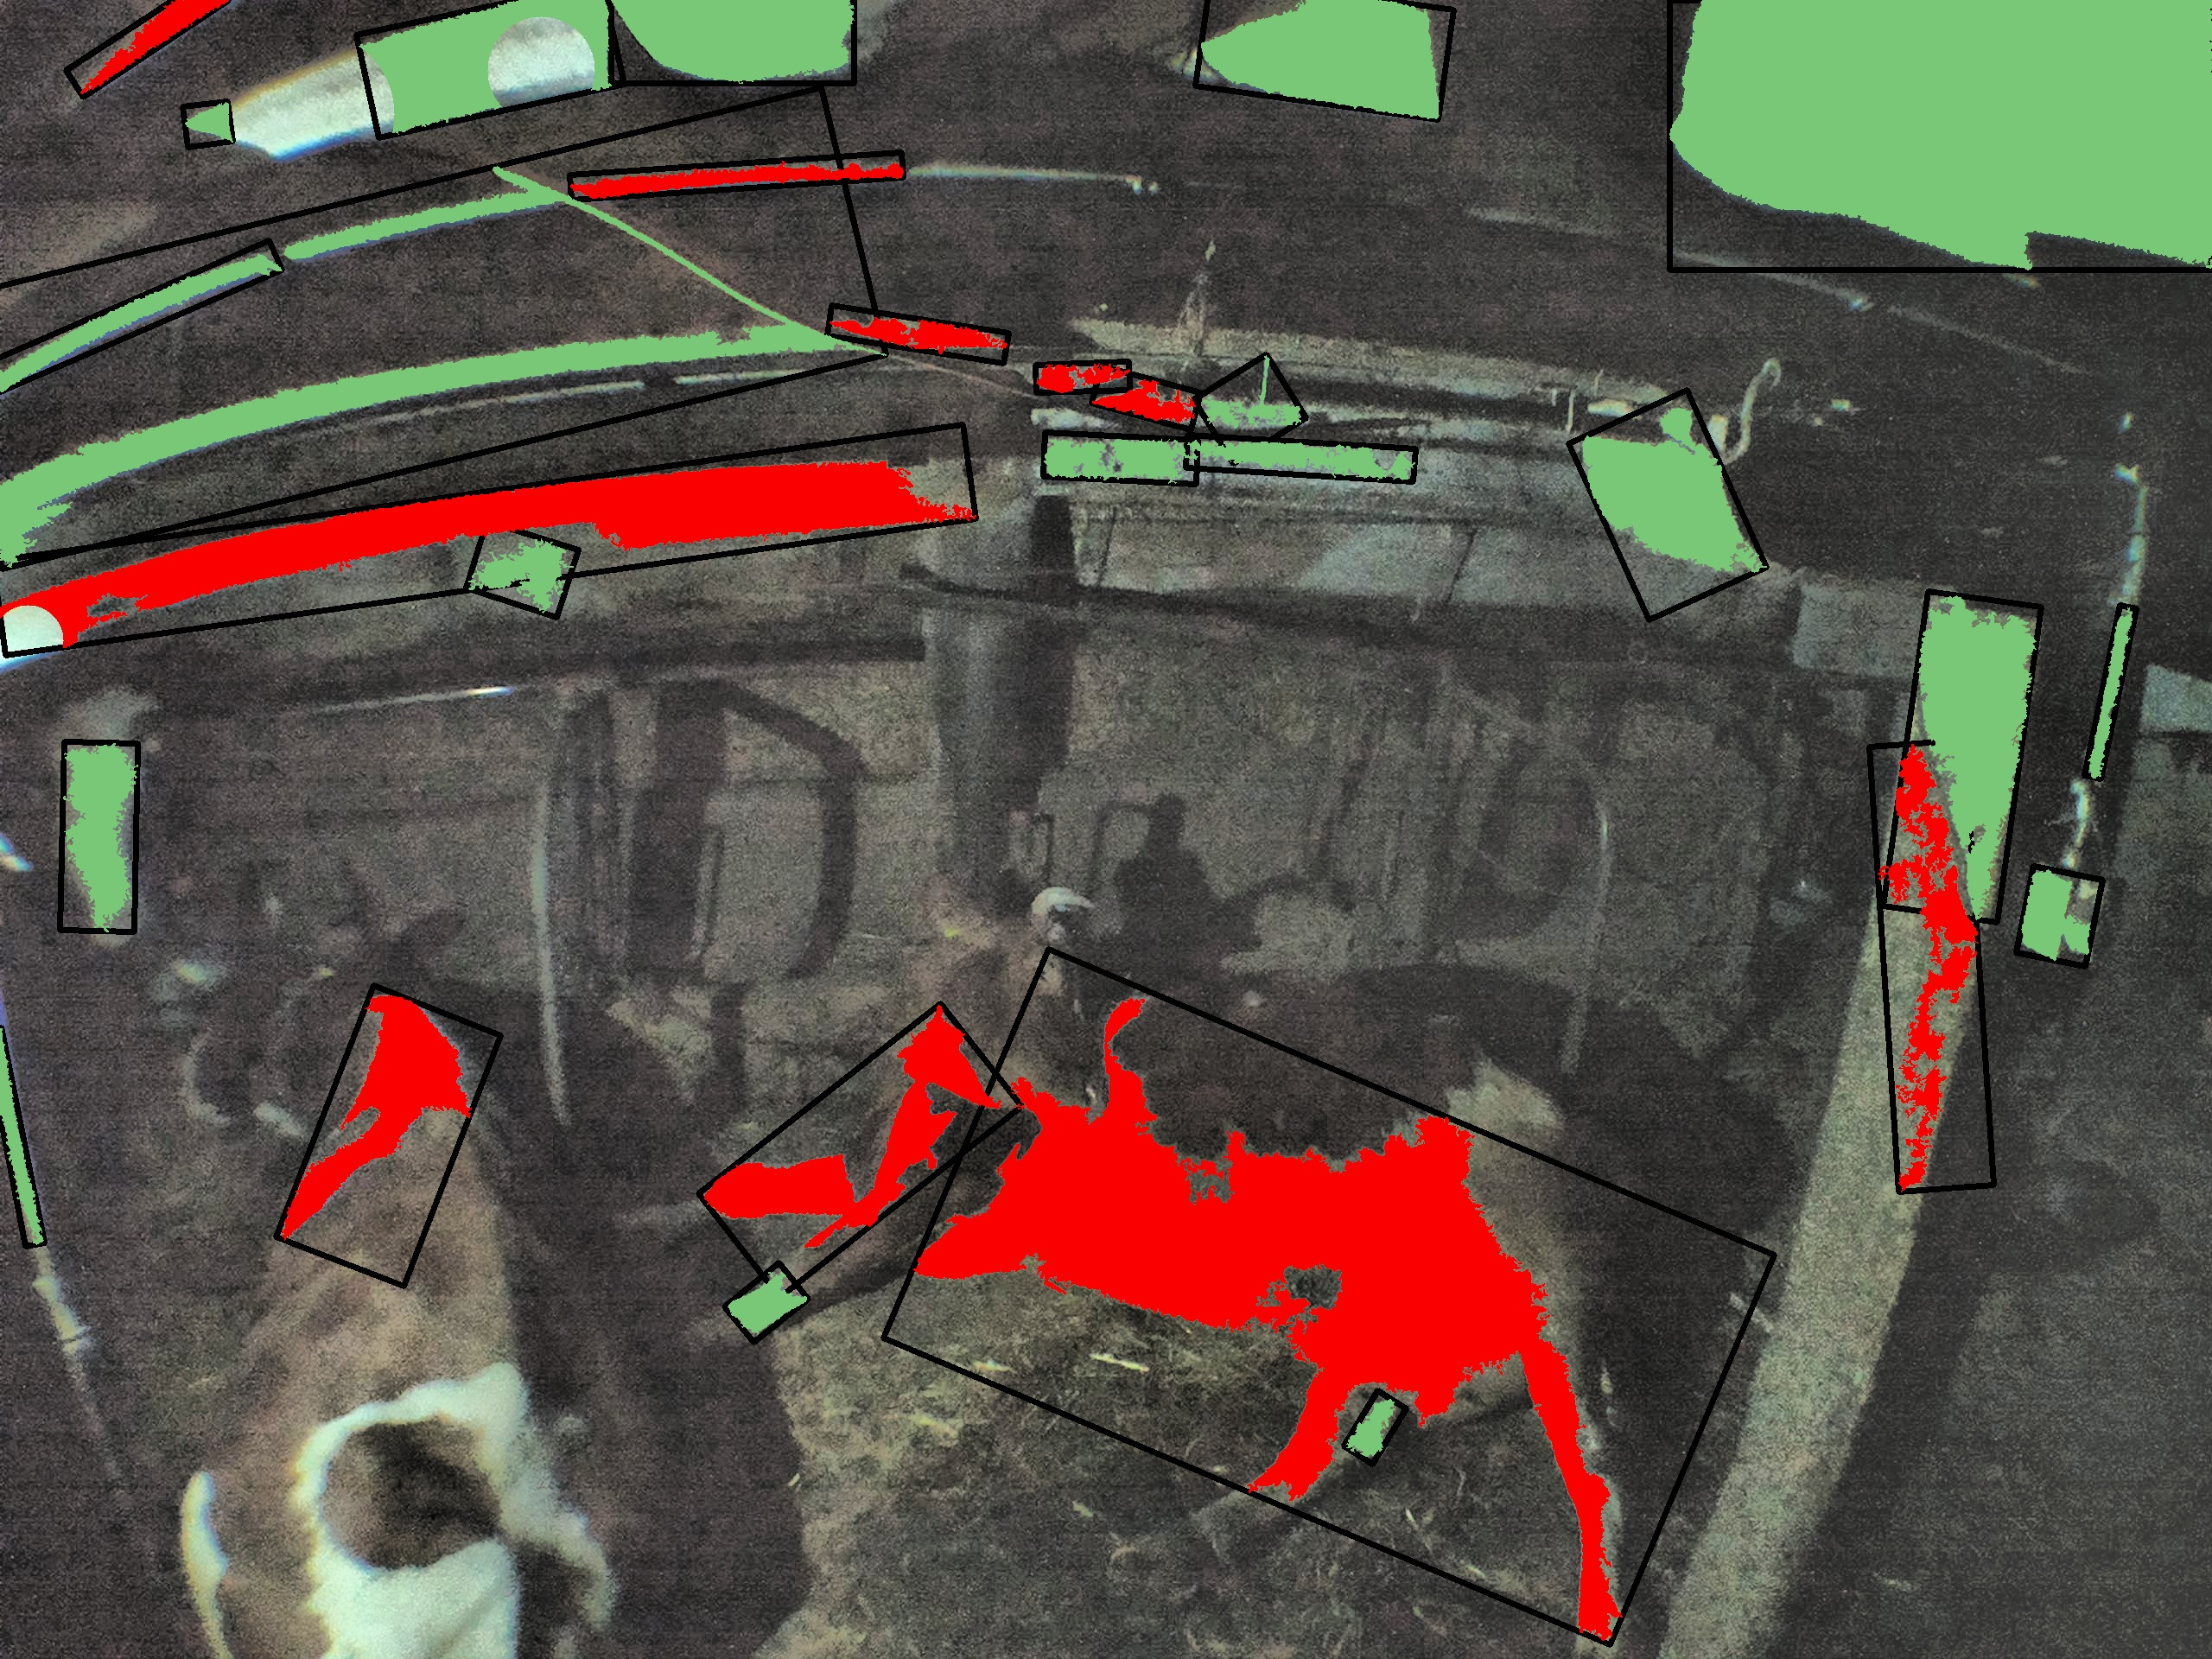
\includegraphics[scale=0.1]{Grafiken/resultate/resultatLying2.jpg}
	\caption{Weiteres Ergebnis von seitlich liegender Kuh} 
	\label{fig: Weiteres Ergebnis von seitlich liegender Kuh} 
\end{figure}